%\documentclass[11pt]{scrartcl}
\documentclass[11pt]{scrreprt}

\usepackage[T1]{fontenc}
\usepackage[utf8]{inputenc}
% \usepackage[ngerman]{babel}

\usepackage{graphicx}
\graphicspath{ 
	{../resources/imgs/},
	{../../data/plots/},
	{../../data/plots/dataset_evaluation/}
}

%\usepackage[backend=biber, style=ieee]{biblatex}
\usepackage[backend=bibtex, style=authoryear-comp]{biblatex}
%\newcommand{\citep}{\parencite}  % adds \citep alias for citing with parenthesis
\let\citef\cite  % makes \citef an alias for \cite
\let\cite\parencite  % makes \cite an alias for \parencite
\addbibresource{../resources/MA.bib}

\KOMAoptions{parskip=half}

\usepackage[margin=3cm]{geometry} % Adjust margins

\usepackage{soul}
\usepackage{todonotes}
\usepackage{amsmath}
\usepackage{hyperref}
\usepackage{cleveref}
\usepackage{caption}
\usepackage{subcaption}
\usepackage{booktabs}
\usepackage{rotating}
\usepackage{pdfpages}
\usepackage{csquotes}
\usepackage{algorithm}
\usepackage{newfloat}
\usepackage{enumitem}
\usepackage{algpseudocode}
\usepackage[export]{adjustbox}

%\usepackage{array}  % needed for '\newcolumntype' command
%\newcolumntype{L}[1]{>{\raggedright\arraybackslash}p{#1}}  % define "L" column type
%% Define a new counter for tracking the list number

% Counter for observation lists
\newcounter{listcounter}
\setcounter{listcounter}{0}

\DeclareFloatingEnvironment[
  listname = {List of Patterns} ,
  name = Pattern,
  placement = h,
  within = none
]{pattern}

\DeclareFloatingEnvironment[
  listname = {List of Hyperedges} ,
  name = Hyperedge,
  placement = h,
  within = none
]{hedge}

\Crefname{pattern}{Pattern}{Patterns}
\crefname{pattern}{pattern}{patterns}
\Crefname{hedge}{Hyperedge}{Hyperedges}
\crefname{hedge}{hyperedge}{hyperedges}


\usepackage{lipsum}  % produces dummy text


\begin{document}


% ========== Title page

\titlehead
{
\begin{tabular}{ll}
\begin{minipage}{0.5\textwidth}
	\textbf{Technische Universität Berlin} \\
	Fakultät IV: Elektrotechnik und Informatik \\
	Institut für Telekommunikationssysteme \\
	Fachgebiet Verteilte offene Systeme	
\end{minipage}
&
\begin{minipage}{0.5\textwidth}
	\raggedleft
	
\includegraphics[width=0.3\textwidth]{logos/tub_logo_bw.jpg}			
\end{minipage}

\end{tabular}
}

\subject{Masters Thesis in Computer Science}
\title{Extending Semantic Hypergraphs by Neural Embedding-based Semantic Similarity for Pattern Matching}
\author{Max Reinhard \\ \small Matrikelnummer: 359417}

\date{\today}
\publishers{Supervised by Prof. Dr. Manfred Hauswirth \\
	Additional guidance by Prof. Dr. Camille Roth\thanks{Centre Marc Bloch (An-Institut der Humboldt-Universität zu Berlin)} \\ 
	and Dipl.-Math. Thilo Ernst\thanks{Fraunhofer-Institut für offene Kommunikationssysteme}}
	
\maketitle

% ========== Abstract
\begin{abstract}
\textbf{Abstract}
\lipsum[1-2]
\end{abstract}

% ========== TOC
\tableofcontents
\newpage

% ========== Body
% ==============================

% ========== 
\chapter{Introduction}
\begin{itemize}
	\item Context: The big problem
	\item Problem statement: The small problem
	\item Methodology / Strategy
	\item Structure
\end{itemize}

\textbf{Notes:}
\begin{itemize}
	\item Huge amounts of text, which can provide insight about stuff
	\item Automatic tools can provide assistance for humans to process all the text
	\item This generally means filtering the original text corpus or otherwise reducing amount of information the information that has to be processed by humans
	\item Filtering introduces a bias
	\item Especially for scientific purposes it is relevant to mitigate bias or at least understand what bias has been introduced (to make it transparent)
	\item Semantic Hypergraphs can be a valuable tool for that because...
\end{itemize}


Human life in times of widespread use of the internet and smartphones is most certainly more than ever interspersed with text-based communication...

Great progress has been made in the made in NLP, IR and IE in the past decade. This advancement of the state-of-the-art can primarily be attributed \textit{Deep Learning} based methods, often also referred to as \textit{Neural Networks}. \cite{youngRecentTrendsDeep2018, minRecentAdvancesNatural2023, hirschbergAdvancesNaturalLanguage2015}

\section{References from the Future}
open-opaque / strict-adaptive categorisation dimensions

\section{Expose intro}

A significant part of the social world is nowadays being represented by digitally manifested text. Examples for this range from instant messaging, social media and any form of collective web activity to encyclopaedic websites, digitized libraries and government intelligence. The amount and richness of available social text makes it a valuable data source for social science research while simultaneously creating an interest in automatic systems to analyze these texts on a large scale \cite{evansMachineTranslationMining2016}. Such research can be understood as part of the domain of \textit{Computational Social Science} (CSS) \cite{lazerComputationalSocialScience2009}.

Systems based on techniques from the field of \textit{ Natural Language Processing} (NLP), as well well as the interlinked fields of \textit{Information Retrieval} (IR) and \textit{Information Extraction} (IE), have demonstrated great success in a variety of task related to text analysis. This success is largly attributed to the advancements of applying of \textit{Machine Learning} (ML) and especially \textit{Deep Learning} (DL) methods to text \cite{hirschbergAdvancesNaturalLanguage2015} \cite{qiuPretrainedModelsNatural2020}. While being very effective at predicting or decision making, ML- and specifically DL-based systems generally do not deliver an explanation for their judgement and can mostly be viewed as "black box models" that are not transparent in their prediction or decision making process \cite{rudinStopExplainingBlack2019}. Conversely this transparency and explainability is of high interest in CSS applications such as predicting political opinion based on social media activity \cite{wilkersonLargeScaleComputerizedText2017}.
%DL models 

The \textit{Semantic Hypergraph} (SH) \cite{menezesSemanticHypergraphs2021} is a framework for representing and analyzing Natural Language (NL). \textit{NL} sentences can be modelled as an ordered, recursive hypergraph which can be represented in a formal language. The framework allows to specify semantic patterns in this formal language which can be matched against an existing SH. It aims to provide an \textit{open} and \textit{adaptive} system to analyse text corpora, especially in the domain of CSS. The framework is \textit{open} in the sense that its representation formalism is inspectable and intelligible by humans and that the pattern matching follows explicit rules. The framework is adaptive in the sense that the parsing is built from adaptive, ML-based subsystems and therefore allows for an error-tolerant parsing from \textit{NL} to \textit{SH} in regards to grammatical and syntactical correctness.



% ========== 
\chapter{Fundamentals and Related Work}
\section{Semantic Hypergraph}

\subsection{Structure}

synonymes: SH, hypergraph, graph.

Edge

Edge Content

Root edge / Sequencen (i use the term "sequence root edge")

\subsection{Syntax / Pattern Matching}

wildcard operator

Variables

Square bracket notation --> word lists

functional patterns -> lemma

> operator for innermost atom


---

Differences between the formal notation and the notation sued in the implementation
(or should this be contained in the implementation chapter?)





\section{Semantic Similarity}

\subsection{Different Similarity Measures}

\subsubsection{String Similarity}
Lievenstein distance, etc..

\subsubsection{Lexical Similarity}
tf-idf, etc.?

\subsection{Types of Semantic Similarity}

\subsubsection{Lexical Databases}
WordNet and alike (not the scope of this work)


\section{Embedding-based Similarity}

\subsection{Embedding Types}

\subsubsection{Fixed Word Embeddings}

\subsubsection{Contextual Ebeddings}

%\subsubsection{Sentence embeddings}

\subsection{Distance Measures}

Mean reference vector vs. pairwise distance

similarity threshold (ST)

% ========== 
\chapter{Problem Statement}
\label{cha:problem-statement}
CSS researches may typically be interested in extracting statements of a specific kind from a text corpus, such as expressions of sentiment of an actor towards some entity or expressions of conflicts between different actors. Two sensible ways to frame this task are as \textit{text classification} \cite{kowsariTextClassificationAlgorithms2019} or \textit{text retrieval} \cite{manningIntroductionInformationRetrieval2008}. It can be addressed with a wide range of system, which will be generally referred to as  \textit{automatic text analysis} systems in the following. These systems are mostly based on techniques from the field of Natural Language Processing (NLP), as well well as the interlinked fields of Information Retrieval (IR) and Information Extraction (IE) \cite{chowdharyNaturalLanguageProcessing2020}.

A relevant perspective of categorising text analysis systems, especially from the point of view of CSS researchers, are the dimensions \textit{open}-\textit{opaque} and \textit{adaptive}-\textit{strict} \cite{menezesSemanticHypergraphs2021}. Here openness refers to the systems users ability to inspect and understand the processing, which we can also bee describes as transparency and explainability. These properties are of high interest in CSS applications such as predicting political opinion based on social media activity \cite{wilkersonLargeScaleComputerizedText2017}. An adaptive text analysis system does not (only) operate on strict rules, but is able to learn and modify its behaviour in some way. It is therefore in principle able to handle unforeseen variations in the text it processes. While both of these two properties are desirable for users are often found to be a trade-off. Current successful adaptive systems are most often bases on neural networks \cite{hirschbergAdvancesNaturalLanguage2015}, which are opaque in the way how they represent and process text \cite{rudinStopExplainingBlack2019}. 

The Semantic Hypergraph (SH) framework aims to fulfil both the open as well as the adaptive property of a text analysis system. It offers an inspectable and understandable representation of text that is constructed by a parser based on machine learning components. The SH representation and its construction can be therefore considered to fulfil the open-adaptive properties. The SH pattern matching language can be used to define patterns that match a specific subset of hyperedges in a given hypergraph. The matching process is purely symbolic and follows a set of fixed rules. It can therefore be considered to be open-strict. In the context of the SH framework the CSS research task described above is better framed as text retrieval. The SH pattern acts  as a \textit{query} for which the most relevant items are retrieved. While the SH frameworks capabilities are not restricted to text retrieval, the work is focused on this application.

The SH pattern defined by a user may among other things specify the structure of the edges that should match it as well as their type (and the types of possible sub-edges). The SH pattern language allows it to describe different levels of generalisations for the structural matching. Additionally the actual words that should match need to be specified i.e. the edge content to match against, if the edge matches the pattern structurally. These words need to be given explicitly and the only way of generalising is via the lemma functional pattern. This lack of generalisation capability entails that a bias is introduced into the matching process by the manual selection of words by the SH frameworks user, who defines the pattern.

%One approach for performing the retrieval would be to use a system which allows to specify some form of pattern which abstractly represents the statements they are trying to capture. This requires the definition of some form of formal pattern language\footnote{The \textit{Google Search} query language can be seen as a simple example of such a pattern language, albeit with a different use case focus: \url{https://support.google.com/websearch/answer/2466433?hl=en}} and possibly the prior transformation of the text corpus into some form of structured format to match against. Another approach is to use a system, which accepts example statements concretely representing the statements that are desired to be retrieved. Those systems may require a large number of positive and negative examples to be able to perform the retrieval. The two types of retrieval systems described here are in tendency situated in the realms of symbolic IR/IE and probabilistic ML/DL respectively.

%The SH framework is more situated in the former symbolic realm. In SH text is represented in the form of \textit{hyperedges} (in the following also referred to as \textit{edges} only). These edges are either atomic or they consist of edges themselves, which essentially accounts for the recursive character of the SH. Each edge has a specific \textit{type} from a set of eight different types of which the most trivial two types are probably \textit{concept} (\textsf{C}) and \textit{predicate} (\textsf{P}). 

%There are additional operators in the pattern language such as the wildcard operator \textsf{*}, which can be used e.g. to match every atomic edge of a specific type and therefore discard content.

To better illustrate the problem \cref{hed:ann-likes-bananas} and \cref{hed:ann-likes-apples} demonstrate how NL sentences are parsed to SH based on this simplified introduction the the SH representation.

\begin{hedge}
  \normalfont\sffamily
  \centering
  ( likes/P ann/C apples/C ) 
  \caption{SH representation for the sentence "Ann likes apples"}
  \label{hed:ann-likes-apples}
\end{hedge}

\begin{hedge}
  \normalfont\sffamily
  \centering
  ( likes/P ann/C bananas/C ) 
  \caption{SH representation for the sentence "Ann likes bananas"}
  \label{hed:ann-likes-bananas}
\end{hedge}

\cref{hed:ann-likes-apples} and \cref{hed:ann-likes-bananas} both follow the same structure, but differ in the content of the last sub-edge. Both edges are hence matched by \cref{pat:ann-likes-something}, which does not specify content for this sub-edge.
The SH pattern language also allows to define a pattern that matches both \cref{hed:ann-likes-apples} and \cref{hed:ann-likes-bananas} via a list of words as in \cref{pat:ann-likes-apples-and-bananas}. However is not possible define a pattern that matches based on some form of \textit{Semantic Relatedness} (SR) or \textit{Semantic Similarity} (SS) \cite{harispeSemanticSimilarityNatural2015} regarding content.
Referring to the example above this means using the SH framework it is not directly possible to to retrieve every sentences that declares that "Ann likes \textit{some kind of fruit}" or that "Ann likes \textit{fruits similar to apples}". This former would require to provide a comprehensive list of every fruit while the latter would require the user to specify all fruits he deems similar to apples.

\begin{pattern}[h!]
  \normalfont\sffamily
  \centering
  ( likes/P Ann/C */C )
  \caption{"Ann-likes-something" pattern}
  \label{pat:ann-likes-something}
\end{pattern}

\begin{pattern}[h!]
  \normalfont\sffamily
  \centering
  ( likes/P ann/C [apples, bananas]/C )
  \caption{"Ann likes apples or bananas" pattern}
  \label{pat:ann-likes-apples-and-bananas}
\end{pattern}

Utilizing some form of SR/SS regarding to edge content in the SH matching process would allow users to define patterns, which describe generalisations of edge content. There exists a great variety of approaches for determining the SR/SS of text, which can generally be divided into \textit{Corpus-based Measures} and \textit{Knowledge-based measures} \cite[Section~1.3.2]{harispeSemanticSimilarityNatural2015}. The latter approaches may generally provide the openness in the measurement determination that is desired by CSS researchers. However among the former recent ML-based and especially DL-based approaches have been outperforming most other approaches \cite{chandrasekaranEvolutionSemanticSimilarity2021}. They generally rely on computing a vector space representation (or embedding) of texts which can then be used to calculate their similarity and will therefore be referred to as neural embedding-based semantic similarity (NESS) measures.

Word semantics generally depend on textual context and hence does the SS between words \cite[Section~2.2.3]{harispeSemanticSimilarityNatural2015}. Incorporating contextuality when extending the SH pattern matching process by SS therefore poses a central challenge. Context-dependent SS would allow to specify matching edge content beyond isolated word semantics, although this may not always be desirable or necessary as in the example above. 

\todo[inline]{
This has to be adapted based on chapter 2 \\
-> add reference to FNESS/CNESS and derive relevancy of both for this work -> modify RQs \\
-> derive in more detail why embedding based SS is chosen \\
-> add discussing about effiency?
}

Integrating NESS measures into the pattern matching process would allow for edge content generalisation and therefore would make the process more adaptive. As illustrated earlier, NESS measures principally do not provide the openness that is inherent to the pattern matching process of the SH framework. In the sense of the open-opaque / strict-adaptive classification described above this integration would mean a shift from openness to opaqueness and from strictness to adaptivity. To counteract the opaqueness introduced by an NESS integration into the SH pattern matching, allowing user control over generalisation levels can maintain some openness while still benefiting from increased adaptivity.

% ========== 
\section{Research Questions}
\label{sec:research-questions}
Based on the problem statement outlined above, we pose the following research questions:

\subsection{Primary Question}
\textbf{R} Can neural embedding-based semantic similarity regarding edge content be be integrated into the pattern matching of the Semantic Hypergraph framework to allow for more generalising patterns while providing control over the generalisation and therefore maintaining some openness of the pattern matching process?

\subsection{Secondary Questions}
\textbf{R.1} What neural embeddings model would be the most suitable for accuratly assessing semantic similarity within the Semantic Hypergraph pattern matching process while effectively addressing the challenges posed by contextuality?

\textbf{R.2} How can neural embedding based semantic similarity effectively (and efficiently?) be integrated into the Semantic Hypergraph pattern matching?

\textbf{R.3} Does integration neural embedding-based semantic similarity improve the retrieval performance of the Semantic Hypergraph framework and how does it impact recall and precision when matching a pattern against a set of known desired matching results?

\textbf{R.4} How can the level of edge content related generalisation in the pattern matching process be effectively and transparently controlled?




% ========== 
\chapter{Solution Approach}
\label{cha:solution-approach}
In this chapter we present the approach that was developed to answer the research questions (see \cref{sec:research-questions}). Therefore trying to provide a solution to the problem of extending the SH framework by Neural Embedding-based Semantic Similarity Matching, which is described in \cref{cha:problem-statement} where the relevancy of this problem for has also been derived.

The system is described here will in the following be referred to as \textit{Neural Embedding-based Semantic Similarity extended Semantic Hypergraph Pattern Matching} or:
\begin{center}
\textit{\textbf{NESS-SHPM}} aka \textit{\textbf{NESSeSHyPaM}}	
\end{center}



The recall of NESS-SHMP in relation to ST \(r(t_s\) is strictly monotonically decreasing, since the set of points in embedding space that is inside of the similarity boundary consistently gets smaller with increasing ST.

\section{Integration into the Pattern Matching Process}
\subsection{SemSim Functional Pattern}
\texttt{semsim} 

pattern works only for atoms

\subsection{Sub-pattern Similarity Thresholds}


\section{Fixed Word Embedding-based Matching}
(FNESS)
 
word2vec via gensim

discussion about using transformer models for single word embeddings?


reference words: single-word and multi-word reference

\label{sec:semsim-multi-word}
Square bracket notation 

\section{Contextual Embedding-based Matching}
\textit{Contextual Neural Embedding-based Semantic Similarity} 
(CNESS)

all tokens option (AT) vs sub tokens


i generally like your idea of contrasting the discrete and continous space as it allows to point out that there cant be one single point, also for a set of words which represents the meaning, but rather some subspace depending on the specific context
Regarding the point of the semantic entities in continuous space being either word- or phrase based, the important difference is, that in case of semsim with context we do not compare the embedding representation of the phrases themselves. rather the sententences/phrases influence the embedding representations of the word (or maybe phrases)
 I tend to see this a bit like a blurring algo. The meaning of each token starts bleeding into its neighbours.


reference edges

\subsection{Context References}
\subsection{Token Mapping}



\section{Similarity Threshold Control}

\subsection{Breakpoint Discovery}
detect change points in number of matches \\ 
see https://github.com/deepcharles/ruptures

half-max point and quarter/three-quarter points (percentiles, not quantiles)
fit function and search for infliction as well as maximum derivative points,
problematic in cases with less continuous change in number of matches.

how to approach this for practical applications?


% ========== 
\chapter{Implementation}
\label{cha:implementation}

\section{Relevant external Software Libraries used}
Here list libs and models to be referenced later.

Word2Vec
Gensim
SentenceTransformers
Transformers
SpaCy

\section{Modules newly added to the SH Framework}
Semsim instances

reference edge sample modification parameter


\section{Modifications of the SH Pattern Matching}
skip semsim

\section{Modifications to the Hypergraph database}
is this really necessary? tok pos etc, but not actually specific to semsim


%\section{SH Notation}
%Bracket notation for multi-word Semsim


%\section{Similarity Threshold}
%\label{sec:similarity-threshold}


%\section{Tokenization}
%
%\subsection{SpaCy}
%SpaCy linguistic tokenization (https://spacy.io/usage/linguistic-features how-tokenizer-works)
%spacy (without transformers) uses an purely rule based (but language depended) tokenizer as far as I understand: https://spacy.io/usage/linguistic-features how-tokenizer-works (the call it linguistic tokenizer)
%
%side note about using different transformer models than the provided one (because i was always confused about this):
%it it possible to exchange the underlying transformer component for basically every transformer model (as long as it follows the conventions that spacy expects), but you would have to retrain the spacy model to be able to use the task specific heads (like e.g. NER)
%footnote: https://github.com/explosion/spaCy/discussions/10327
%
%an alignment is provided between the transformer-tokenizer and the spacy-tokenizer
%lib: https://github.com/explosion/spacy-alignments
%
%footnote: https://explosion.ai/blog/spacy-transformers
%
%
%\subsection{WordPiece and SentencePiece}
%
%SentencePiece: https://github.com/google/sentencepiece


%\section{Matching candidate edge and reference edge tokens}
%both edges should match the pattern and should act as a valid ref edge for each other
%but it is obvious that the tok_idx_trail that leads to the predicate in the one edge wont lead to the predicate in the other edge
%that was the premise on which i built the matching (and which we discussed i think)
%
%so there are 2 cases:
%[candidate edge is more specific than reference edge] the location trail of the token in the candidate edge is longer than in the reference edge. this case should be trivial. we can just cut off the location trail when we reach an atom in the reference tok_pos.
%[reference edge is more specific than candidate edge] the location trail of the token in the candidate edge does not lead to an atom in the reference edge. in this case there is not enough information to match the tokens. i see two possible solutions:
%use the whole sub-edge to compute the reference embedding (maybe i misunderstood and that was your conception all along)
%try to get the information which token to use in some other way. possibly by matching via the atom types… this should work for cases like predicates but would not work if we are looking for a modifier or something else which can appear multiple times. i have the feeling that this should be recoverable through the graphbrain matching process somehow, i just don’t know how….
%(edited)
%
%for now i have the tendency to implement 2a as it is much easier not sure about the semantic implications though




% ========== 
\chapter{Evaluation}
In this chapter the conceived concept (see \cref{cha:solution-approach}) and specific implementation (see \cref{cha:implementation}) of the NESS-SHPM system is being evaluated to answer the research question(s) posed in \cref{sec:research-questions}. Therefore a a case study is conducted to evaluate the system for a specific use case. 
%In this case study...
\todo[inline]{refer to the RQs more specifically? how are they going to be answered?}

\section{Case Study: Conflicts}
The conflicts case study follows the approach presented in \citef{menezesSemanticHypergraphs2021}, where expressions of conflict are extracted from a given SH using a single SH pattern. In their work they build upon the information extracted by the pattern to conduct further analyses, which are not in the scope of this work. Here the evaluation is limited to the task of classifying whether the content of a given edge in the SH is an expression of conflict or not. Or framed differently, the task is to retrieve exactly all those edges whose content is an expression of conflict. The evaluation will compare the retrieval performance of a suitable set of different SH patterns and corresponding configuration of the NESS-SHMP system by matching them against a labelled dataset of hyperedges.

\todo[inline]{should I explain why specifically the conflicts and not some other case study (i.e. dataset) --> because there was none... but then I need to show why there was none and what are the criteria for a case study to be suitable to evaluate the system}

\subsection{Expressions of Conflict}
\label{sec:conflict-definition}
An expression of conflict in the context of this case study is defined as a sentence which fulfils the following properties:

\begin{displayquote}
There is a conflict between two explicitly named actors, wherever these actors are mentioned in the sentence; whereby a conflict is defined as antagonizing desired outcomes.
\end{displayquote}

\subsection{Reddit Worldnews Corpus}
The corpus from which those expressions of conflict are retrieved consists of news titles that were shared on the social media platform \textit{Reddit}. Specifically all titles shared between January 1st, 2013 and August 1st, 2017 on \textit{r/worldnews}, which is described as: “A place for major news from around the world, excluding US-internal news.”\footnote{\url{http://reddit.com/r/worldnews}} This corpus contains 479,384 news headers and is in the following referred to as the \textit{Worldnews-Corpus}.

Each of these headers is comprised of a single sentence and is represented as a sequence root edge in the SH constructed from it. In the following this SH is referred to as the \textit{Worldnews-SH}. Parsing errors that may potentially occur during this constructed and can obstruct a correct retrieval of a wrongly parsed edge i.e. wrongly represented sentence. These errors are out of scope of this work. All edges in the Worldnews-SH are assumed to be correctly parsed.

%These are some randomly selected examples from the Worldnews-Corpus:
%\begin{itemize}
%	\item Example
%	\item Example
%	\item Example
%\end{itemize}
%
%\todo{add examples}


\subsection{Semantic Hypergraph Patterns}
\label{sec:sh-patterns}
The SH patterns that are used in this evaluation all have the same general form to isolate the effect of replacing a purely symbolic matching against a specific word or list of words with NESS-SHMP. In this section the general form of these pattern will be described, which entails consequences for the creation of the labelled dataset described in \cref{sec:conflict-dataset}. 

%The retrieval performance of the original purely symbolic pattern defined by \citef{menezesSemanticHypergraphs2021} is compared against the retrieval performance of patterns containing some form of the semsim functional pattern. \todo{remove?}


\subsubsection{Original Conflict Pattern}
\Cref{pat:original-conflict} is originally defined in \citef[p.~22]{menezesSemanticHypergraphs2021} and is therefore referred to as the \textit{original conflict pattern}. It is used to extract conflicts between two parties \textsf{SOURCE} and \textsf{TARGET}, potentially regarding some \textsf{TOPIC}. As mentioned before, the assignment of these variables is irrelevant for this case study.

The original conflict patterns contains two sub-patterns which utilize word lists. These sub-patterns match the trigger sub-edge and predicate sub-edge of a candidate edge respectively and are in following referred to as \textit{trigger sub-pattern} and \textit{predicate sub-pattern}. If not stated otherwise these terms will refer to \cref{pat:original-conflict}. 

\begin{itemize}
	\item \textbf{\textsf{Trigger sub-pattern:}} \textsf{[against,for,of,over]/T}
	\item \textbf{\textsf{Predicate sub-pattern:}}
		\textsf{( PRED/P.{so,x} ) \(\wedge\) \\ ( lemma/J >PRED/P [accuse,arrest,clash,condemn,kill,slam,warn]/P )}
\end{itemize}

In the trigger sub-pattern the content of the candidate trigger sub-edge is directly matched against a list of prepositions, which are in the following referred to as the \textit{conflict prepositions}. In case of the predicate sub-pattern, the word list is matched against the lemma of the innermost atom of the candidate predicate sub-edge, which is always a verb. The list of verbs used here will in the following be referred to as the \textit{conflict verbs}.

\begin{itemize}
	\item \textbf{\textsf{Conflict prepositions:}} against, for, of, over
	\item \textbf{\textsf{Conflict verbs:}} accuse, arrest, clash, condemn, kill, slam, warn
\end{itemize}


\begin{pattern}
  \normalfont\sffamily
  \centering
  ( PRED/P.{so,x} SOURCE/C TARGET/C [against,for,of,over]/T TOPIC/[RS] ) \(\wedge\) \\
  ( lemma/J >PRED/P [accuse,arrest,clash,condemn,kill,slam,warn]/P )
  \caption{Original conflict pattern}
  \label{pat:original-conflict}
\end{pattern}


\subsubsection{Wildcard Conflict Patterns}
\label{sec:wildcard-conflict-patterns}
Replacing either the trigger sub-pattern, the predicate sub-pattern or both of them with a semsim function are the options for utilizing NESS-SHPM in a modified version of \cref{pat:original-conflict} without modifying the general structure of the pattern. To evaluate which of these options are best suited to evaluate the retrieval performance of NESS-SHPM, three \textit{wildcard conflict patterns} are constructed. In these patterns the predicate sub-pattern (\cref{pat:wildcard-pred}) or the trigger sub-pattern (\cref{pat:wildcard-prep}) are replaced by the wildcard operator. 
%or both (\cref{pat:wildcard-pred-prep})

\begin{pattern}
  \normalfont\sffamily
  \centering
  ( PRED/P.{so,x} SOURCE/C TARGET/C [against,for,of,over]/T TOPIC/[RS] ) \(\wedge\) \\ ( PRED/P */P )
  \caption{Predicate wildcard pattern}
  \label{pat:wildcard-pred}
\end{pattern}

\begin{pattern}
  \normalfont\sffamily
  \centering
  ( PRED/P.{so,x} SOURCE/C TARGET/C */T TOPIC/[RS] ) \(\wedge\) \\  ( lemma/J >PRED/P [accuse,arrest,clash,condemn,kill,slam,warn]/P )
  \caption{Trigger wildcard pattern}
  \label{pat:wildcard-prep}
\end{pattern}

%\begin{pattern}
%  \normalfont\sffamily
%  \centering
%  ( */P.{so,x} SOURCE/C TARGET/C */T TOPIC/[RS] )
%  \caption{Predicate and trigger wildcard pattern}
%  \label{pat:wildcard-pred-prep}
%\end{pattern}

\paragraph{Preliminary Evaluation}
The three wildcard conflict patterns are matched against the Worldnews-SH and the number of matches is recorded. Comparing the number of matches of these patterns shows which of the sub-patterns is most influential for the retrieval performance of \cref{pat:original-conflict}. \Cref{tab:wildcard-pattern-evaluation} shows the results of these preliminary evaluations as well as the number of matches that result from matching \cref{pat:original-conflict} against the Worldnes-SH. It can be seen that the choice of conflict verbs is much more influential on the number of matches than the choice of conflict prepositions when compared to the number of matches resulting from the original conflict pattern. While replacing the predicate sub-pattern with a wildcard operator yields an increase with a factor of \(12,45\), replacing the trigger sub-pattern with a wildcard operator only yields and increase with a factor of \(1,07\). 


\begin{table}[h]
\centering
\begin{tabular}{lr}
\toprule
\multicolumn{1}{l}{Pattern name}				& \multicolumn{1}{l}{Number of matches} \\
\midrule
Original conflict pattern					& 5766	\\
Predicate wildcard pattern					& 71804 \\
Trigger wildcard pattern						& 6154	\\
%Predicate and trigger wildcard pattern		& 79431	\\
\bottomrule
\end{tabular}
\caption{Results of matching the wildcard patterns against the Worldnews-SH}
\label{tab:wildcard-pattern-evaluation}
\end{table}



\subsubsection{SemSim Conflict Patterns}
Based on the result of the preliminary evaluation in \cref{sec:wildcard-conflict-patterns}, the predicate sub-pattern of \cref{pat:original-conflict} is replaced by different forms of semsim functional patterns to construct different \textit{semsim conflict patterns}. These patterns are then used to evaluate the effects of utilizing NESS-SHPM. The trigger sub-pattern is not modified to better isolate these effects in comparison to purely symbolic SHPM.

\Cref{pat:semsim-conflict} describes the general form of a semsim conflict pattern. The \texttt{<SEMSIM-FUNCTION>} placeholder is replaced with one of the three implemented semsim functions to construct the \textit{semsim-fix conflict pattern} (\cref{pat:semsim-fix-conflict}), \textit{semsim-fix-lemma conflict pattern} (\cref{pat:semsim-fix-lemma-conflict}) and the \textit{semsim-ctx conflict pattern} (\cref{pat:semsim-ctx-conflict}). As \texttt{<SEMSIM-ARGUMENT>} the conflict verb list is used as similarity reference words in \cref{pat:semsim-fix-conflict} and \cref{pat:semsim-fix-lemma-conflict}, which utilize FNESS. In the semsim-ctx conflict pattern, the wildcard operator is used as \texttt{<SEMSIM-ARGUMENT>} since the necessary reference edges can only be provided via an external parameter and not inside the pattern.


\begin{pattern}[H]
  \normalfont\sffamily
  \centering
  ( PRED/P.{so,x} SOURCE/C TARGET/C [against,for,of,over]/T TOPIC/[RS] ) \(\wedge\)\\ 
  ( \texttt{<SEMSIM-FUNCTION>}/J PRED/P \texttt{<SEMSIM-ARGUMENT>}/P )
  \caption{General SemSim conflict pattern}
  \label{pat:semsim-conflict}
\end{pattern}

\begin{pattern}[H]
  \normalfont\sffamily
  \centering
  ( PRED/P.{so,x} SOURCE/C TARGET/C [against,for,of,over]/T TOPIC/[RS] ) \(\wedge\)\\ 
  ( semsim/J PRED/P [accuse,arrest,clash,condemn,kill,slam,warn]//P )
  \caption{semsim-fix conflict pattern}
  \label{pat:semsim-fix-conflict}
\end{pattern}

\begin{pattern}[H]
  \normalfont\sffamily
  \centering
  ( PRED/P.{so,x} SOURCE/C TARGET/C [against,for,of,over]/T TOPIC/[RS] ) \(\wedge\)\\ 
  ( semsim-fix-lemma/J PRED/P [accuse,arrest,clash,condemn,kill,slam,warn]//P )
  \caption{semsim-fix-lemma conflict pattern}
  \label{pat:semsim-fix-lemma-conflict}
\end{pattern}

\begin{pattern}[H]
  \normalfont\sffamily
  \centering
  ( PRED/P.{so,x} SOURCE/C TARGET/C [against,for,of,over]/T TOPIC/[RS] ) \(\wedge\)\\ 
  ( semsim-ctx/J PRED/P */P )
  \caption{semsim-ctx conflict pattern}
  \label{pat:semsim-ctx-conflict}
\end{pattern}



\section{Conflict Dataset}
\label{sec:conflict-dataset}
To conduct an evaluation which assesses the retrieval performance of the NESS-SHPM system it is necessary to have a dataset of edges with labels that state whether an edge is an expression of conflict or not. Since such a dataset does not exists it needs to be constructed. In the following the construction process of this \textit{conflict dataset} (CD), which is used for the evaluation in this case study, and the datasets characteristics are discussed.


\subsection{Base Edge Set}
\label{sec:base-edge-set}
The set of edges that can be retrieved by a conflict pattern, i.e. the original conflict pattern or a semsim conflict pattern is restricted the general form of these patterns. This entails that, given the same SH, every set of matching edges of a pattern of this form will be a subset of the matching edges of the predicate wildcard pattern (\cref{pat:wildcard-pred}). The set of edges resulting form matching this pattern against the Worldnews-SH are therefore used as the \textit{base edge set} (BES) from which the conflict dataset is constructed, instead of the entirety of all the hypergraphs sequence root edges.

\paragraph{Predicate Lemma} Every edge in the BES has a predicate sub-edge that has an innermost atom, which is a verb that has a lemma. In the following this is called the \textit{predicate lemma} of an edge. Each of the edges matching \cref{pat:original-conflict} or a pattern in the form of of \cref{pat:semsim-conflict} therefore corresponds to a predicate lemma.

%Matching \cref{pat:wildcard-pred} against the Worldnews-SH results in \(n_{f} = 69 380\) matching edges. In the following the set of those edges will be referred to as the \textit{BSE} (FD).\todo{add examples}

\subsection{Desired Characteristics}
\label{sec:dataset-characteristics}
To effectively evaluate the effectiveness of the application of NESS by matching a pattern in the form of \cref{pat:semsim-conflict}, the dataset used for this should have the following characteristics:

\begin{itemize}
	\item Contain the largest possible number of unique predicate lemmas
	\item Contain the largest possible number of edges per unique predicate lemma
\end{itemize}

On the one hand it is desired to have as many different unique predicate lemmas as possible in the dataset to be able to evaluate whether NESS can differentiate if a predicate lemma indicates an expression of conflict or not. On the other hand it is desired to have as many different edges per unique lemma as possible in the dataset to be able to evaluate whether CNESS is able to differentiate if edges represent an expression of conflict or not, given that they correspond to the same predicate lemma.

\subsection{Construction Process}
To create the labelled CD, the edges of the dataset need to be manually labelled by human annotators, which is labor-intensive. The BES contains \(n_b=71804\) edges. Due to the time constrains of this work and the limited availability of three annotators, the BES needs to be subsampled to create the CD. 

\subsubsection{Filtering}
Since the desired characteristics described above relate the the distribution of predicate lemmas, it is relevant to verify that is possible to determine the predicate lemma for all edges in the edge set from which the CD is sampled. In some cases it is not possible to determine the predicate lemma of a given edge due to to implementation issues, which out of scope of this work. In these cases an edge is filtered from the BES, which results in the \textit{filtered base edge set} (FBES). The FBES contains \(n_{f} = 69 380\) edges. 


\subsubsection{Sampling} 
The edges in the FBES correspond to \(n_{l} = 2195\) unique predicate lemmas. Attaining to the desired dataset characteristics, the number of samples \(n_{s}\) in the subsampled dataset should ideally be a multiple \(m_{l} >= 2\) of \(n_{l}\), so that \(n_{s} = m_{l} \cdot  n_{l}\). This would mean that every predicate lemma contained in the FBES is statistically represented multiple times in the subsampled dataset.

A dataset size of \(n_{s}=2000\) was chosen, wich means \(m_{l} < 2\) and  \(n_s << n_f\). This entails that a trade-off between the desired dataset characteristics has to be made. To account for this, a sampling method is applied that offers more control over the distribution of predicate lemmas in the subsampled dataset than uniform random sampling does. This sampling method is based on the idea of \textit{Stratified Sampling} \cite{parsonsStratifiedSampling2017} \todo{is this correct?} and is described in detail in \cref{algo:dataset-sampling}. 

The procedure splits the FBES into multiple bins after the edges are sorted by number of occurrence of their predicate lemma and then uniformly randomly samples from each bin. This method guarantees that predicate lemmas which correspond to a relatively small number of edges in the FBES will be represented in the subsampled dataset. The distribution of uniques lemmas in the FBES and the CD is compared visually in \cref{fig:dataset-lemma-distribution}.

\begin{figure}
\centering
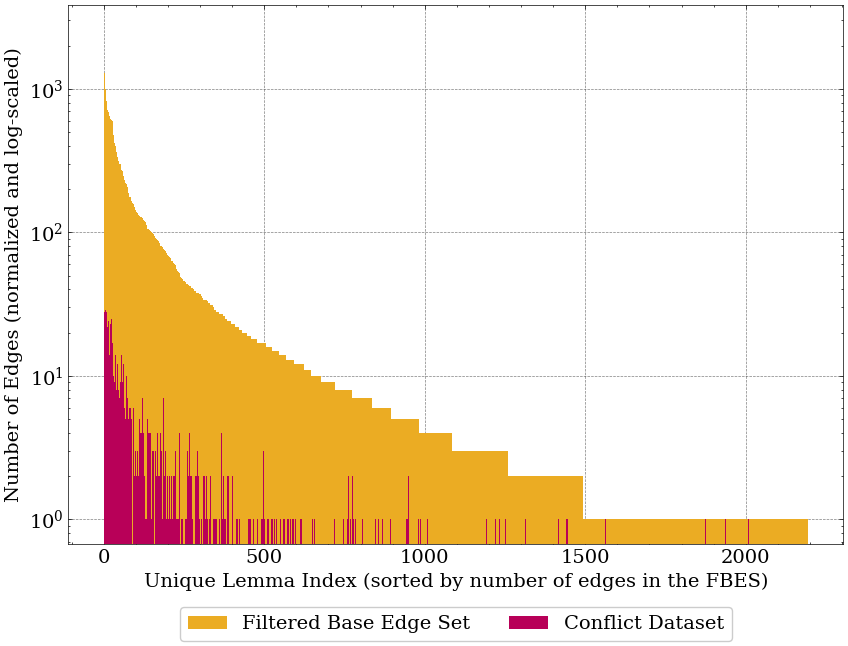
\includegraphics[width=0.8\textwidth]
{dataset_lemma_distribution/lemma_distribution_dataset_conflicts_1-2_pred_wildcard_full_dataset_conflicts_1-2_pred_wildcard_subsample-2000.png}
\caption{Distribution of unique lemmas in the FBES and CD}
\label{fig:dataset-lemma-distribution}
\end{figure}


\begin{algorithm}
\begin{enumerate}
	\item Create a list of tuples \(t\) of edges and their corresponding predicate lemma: \\ \(L = [(l_k, e_i), ...]\) with \(k \in \{0,...,m\}\) and \(i \in \{0,...,n\}\)
	\item Sort this list by the number of tuples containing a predicate lemma to create the list: \\ \(L_{sort} = [(l_0, e_0), ... (l_m, e_n)]\), so that:
	\begin{itemize}
		\item \(n_k\) is the number of tuples containing a lemma \(l_k\)
		\item \(t_j\) with \(j > i\) is a tuple wich sorted after tuple \(t_i\)
		\item \(n_o >= n_p\) if \(t_i = (l_o, e_i)\) and \(t_j = (l_p, e_j)\)
	\end{itemize}			
	\item Split the list \(L_{sort}\) into \(n_{b}\) bins.
	\item Uniformly sample \(n_{sb}\) tuples from each bin.
	\item Build a set of all edges \(e\) contained in the sampled tuples.
\end{enumerate}
\caption{Dataset sampling algorithm}
\label{algo:dataset-sampling}
\end{algorithm}

The subsampled dataset size resulting from this sampling method is \(n_{s} = n_{b} * n_{sb}\). Given \(n_{s} = 2000\), the values \(n_b = 10\) and \(n_{sb} = 200\) were chosen for sampling the CD.


\subsubsection{Labelling}
The labelling task is shared between the three annotators. A given edge will be either labeled as \textit{conflict} or \textit{no conflict} by an annotator following the definition given in \cref{sec:conflict-definition}. Because of the aforementioned time constraints, every edge is only labeled by one annotator. To nonetheless ensure a consistent labelling among all annotators, a set of 50 edge is labelled by all three annotators. Every edge for which a disagreement in labelling occurs between at least two of the annotators, is inspected to reach an agreement on the label. Utilizing this process, the annotators understanding of what constitutes an expression of conflict is refined. Following this preliminary step, the \(n_s\) edges of the dataset are equally distributed among the three annotators and individually labelled by them.

% It was confirmed that the percentage of edges that represent an expression of conflict in relation to all edges in the subset given to an annotator did not vary more than ... among all three annotators.

\subsection{Edge Set Comparison}
The CD is the result of the filtering, sampling and labelling described above. The size of the Worldnews-SH, BES, FBES and CD are listed in \cref{tab:dataset-descriptions} for comparison. If applicable the the number of unique lemmas as well as the number and percentage of edges which are labelled as an expression of conflict and of those which are not are also noted.\todo{add examples? (in appendix?)}


\begin{table}
\centering
\begin{tabular}{lrrrr}
\toprule
\multicolumn{1}{l}{Edge set name}	& \multicolumn{1}{c}{Number of} & \multicolumn{1}{c}{Number of}		& \multicolumn{1}{c}{Number of} 		& \multicolumn{1}{c}{Number of} \\
\multicolumn{1}{l}{} 				& \multicolumn{1}{c}{all edges} & \multicolumn{1}{c}{un. lemmas}			& \multicolumn{1}{c}{conflict edges} 	& \multicolumn{1}{c}{no conflict edges} \\
\multicolumn{1}{l}{} 				& \multicolumn{1}{c}{} 			& \multicolumn{1}{c}{}				& \multicolumn{1}{c}{(\% of all edges)} & \multicolumn{1}{c}{(\% of all edges)} \\
\midrule
Worldnews-SH						& 479384		& -			& -					& - \\
Base Edge Set (BES)					& 71804		& -			& -					& - \\
Filtered BES (FBES)					& 69380 		& 2195 		& - 					& - \\
Conflict Dataset (CD)				& 2000 		& 539 		& 599 (29.95 \%) 	& 1401 (70.05 \%) \\
\bottomrule
\end{tabular}
\caption{Number of edges, number of unique lemmas and proportion of labels for the different edge sets}
\label{tab:dataset-descriptions}
\end{table}


\section{Evaluation Process}
In this evaluation multiple \textit{evaluation runs} are conducted. Each evaluation run correspond to a SHPM process in which a pattern is matched against the CD. In the case of patterns utilizing NESS this requires that additional parameters in form of an \textit{NESS configuration} are given to the matching process. An evaluation run is described by an \textit{evaluation (run) configuration}. For each evaluation run the \textit{evaluation metrics} are computed. 

\subsection{Evaluation Run Configurations}
An evaluation configuration consists of the following parameters: \todo{add references to chapter 4}
\begin{itemize}
	\item Conflict Pattern
	\item NESS Configuration (in case NESS-SHMP): 
	\begin{itemize}
		\item NESS model
		\item Similarity Threshold 
		\item Use  all tokens (in the case of CNESS) 
		\item Reference Edge Set (in the case of CNESS) 
	\end{itemize}
\end{itemize}

\paragraph{Conflict Patterns}
The four conflict patterns used in this evaluation are described in detail in \cref{sec:sh-patterns}. An overview of the properties of these patterns can be seen in \cref{tab:evaluation-patterns}.


\paragraph{Similarity Thresholds}
In this evaluation the similarity threshold \(t_s\) is always selected from a range of thresholds \(r_t = \{0, 0.01, ...,  0.99, 1.00\}\), i.e. \(t_s \in r_t\). This results in 101 different values of \(t_s\).


\paragraph{Reference Edge Sets}
Multiple \textit{reference edge sets} (RES)  are randomly sampled from the set of edges in the CD, which are labelled as "conflict". These edges are then excluded from the dataset, to avoid introducing data from the test dataset to the system that is being evaluated. To compare the effect of different sample sizes, differently sized sets are drawn. To compare the effect of different samples, different samples are drawn. A RES with ID \textit{N-X} has \(N \in \{1, 3, 10\}\) samples and is from sample draw \(X \in \{1, 2, 3, 4, 5\}\). This results in 15 different RES in total. The specific sets that have been sampled can be seen in \cref{app-sec:ref-edge-sets}.


\subsubsection{Evaluation Run Names}
\label{sec:eval-run-names}
An evaluation run name has the form: \texttt{CP NM-AT r-N-X t-TS}

%\begin{center}
%\texttt{<CP> <NM>-<AT> <r-N-X> <t-TS>}
%\end{center}
In a specific evaluation run name, the placeholders (capitalised letters) are replaced with actual values. Such a name always begins with the conflict pattern (CP) name in its shortened form: \textit{original}, \textit{semsim-fix}, \textit{semsim-fix-lemma} or \textit{semsim-ctx}. In case of a NESS utilizing conflict pattern, the NESS model (NM) name is added in its shortened form: word2vec as \textit{w2v} and conceptnet-numberbatch as \textit{cn}. If the NESS type is CNESS, the usage of the all-tokens (AT) option is indicated by adding \texttt{-at} to the model name. If the option is not used, it is not added. Also in case of CNESS, the reference edge set ID N-X is indicated by appending \texttt{r-N-X}. For all NESS utilizing evaluation runs, the similarity threshold \(t_s\) is indicated by appending \texttt{t-TS}, where \texttt{TS} is the value of \(t_s\).



\subsubsection{Specification of Evaluation Run Configurations}
\label{sec:evaluation-configurations}
The configurations for all evaluation runs that are conducted in this case study are specified in \cref{tab:evaluation-run-configs}. All possible parameter combinations of an evaluation configuration, i.e. the conflict pattern and the NESS parameters, are evaluated. The total number of conducted evaluation runs therefore amounts to 6465.\footnote{1 (original) + 2 (semsim-fix and semxim-fix-lemma) * 2 (FNESS models) * 101 (STs) \\ + 1 (semsim-ctx) * 2 (CNESS models) * 2 (all tokens) * 15 (ref. edge sets) * 101 (STs)} In \cref{tab:evaluation-run-configs} the different values for the reference edge set ID and the ST are omitted. The \textit{random} evaluation run configuration relates to a hypothetical evaluation run in which edges are uniformly randomly matched. 


\subsection{Evaluation Metrics}
\label{sec:evaluation-metrics}
Using the information provided by the dataset labels it is determined whether a match is correct or not. If an edge is matches in a given evaluation run and is labeled as "conflict" in the dataset, it is considered a \textit{true positive} (TP). If an edge matches but is labeled "no conflict", it is considered a \textit{false positive} (FP). The \textit{true negatives} (TN) and \textit{false negatives} (FN) are determined analogously  by examining the non-matching edges. Based on the TP, FP, TN and FN the metrics \textit{precision}, \textit{recall} and \textit{F1-score} are computed. \todo{show how this metrics are computed?}

\todo[inline]{derive why these metrics were chosen: \\
accuracy is not interesting since the dataset is unbalanced, precision and recall both of interest, but are expected to be a trade-off (where recall should decline with rising ST). F1-score is an established metric that closely relates to precision and recall and represents this trade-off and therefore retrieval performance as a whole. MCC is arguably a better metric because it is symmetrical and incorporates true negatives. also the F1-score of the original pattern is worse than random, which indicates a metric mismatch. then again the close relation and equal value range of precision, recall and F1-score are a plus (for plotting especially).
}


\begin{table}
\centering
\begin{tabular}{lcccc}
\toprule
\multicolumn{1}{l}{Pattern name}		& \multicolumn{1}{c}{Lemma}		& \multicolumn{1}{c}{NESS}	& \multicolumn{1}{c}{Includes}		& \multicolumn{1}{c}{Requires} \\
\multicolumn{1}{l}{} 				& \multicolumn{1}{c}{based} 		& \multicolumn{1}{c}{type} 		& \multicolumn{1}{c}{ref. words} 	& \multicolumn{1}{c}{ref. edges} \\
\midrule
Original conflict pattern (\ref{pat:original-conflict})					& Yes 		& - 		& -			& - \\
semsim-fix conflict pattern (\ref{pat:semsim-fix-conflict})				& No		& Fixed		& Yes		& No \\
semsim-fix-lemma conflict (\ref{pat:semsim-fix-lemma-conflict}) 		& Yes 		& Fixed		& Yes		& No \\
semsim-ctx conflict patter (\ref{pat:semsim-ctx-conflict})				& No		& Contextual	& No		& Yes \\
\bottomrule
\end{tabular}
\caption{Properties of the conflict patterns used in the evaluation}
\label{tab:evaluation-patterns}
\end{table}


\begin{table}
\centering
\begin{tabular}{llcc}
\toprule
\multicolumn{1}{l}{Evaluation Run Name} & \multicolumn{1}{l}{Conflict Pattern} & \multicolumn{2}{c}{NESS Configuration} \\
\cmidrule{3-4}
\multicolumn{1}{l}{}   & \multicolumn{1}{l}{}  & \multicolumn{1}{c}{NESS Model}	& \multicolumn{1}{c}{all tokens} \\
\midrule
original                       & original                     & -                          & -                \\
semsim-fix w2v                 & semsim-fix                   & word2vec                   & -                \\
semsim-fix cn                 & semsim-fix                   & conceptnet-numbatch                      & -      \\
semsim-fix-lemma w2v           & semsim-fix-lemma             & word2vec                   & -                \\
semsim-fix-lemma cn           & semsim-fix-lemma             & conceptnet-numbatch                      & -      \\
semsim-ctx e5 r-N-X                & semsim-ctx                   & e5                         & No           \\
semsim-ctx gte r-N-X              & semsim-ctx                   & gte                        & No            \\
semsim-ctx e5-at r-N-X             & semsim-ctx                   & e5                         & Yes          \\
semsim-ctx gte-at r-N-X           & semsim-ctx                   & gte                        & Yes           \\
\end{tabular}
\caption{Evaluation Run Configurations}
\label{tab:evaluation-run-configs}
\end{table}




\section{Evaluation Results}
\label{sec:evaluation-results}
In this section the results of the evaluation runs which are defined by the evaluation configurations in \cref{sec:evaluation-configurations} are examined. Different perspectives on the result data are constructed in the form of tables and plots to enable answering the research questions. The following subsections each represent one perspective and conclude with significant observations that can be made based on it.

\subsubsection{Result Data Description Concepts}
To facilitate constructing insightful perspectives on the result data, some novel concepts for its description are introduced in the following.

\paragraph{Evaluation Run Sets}
Multiple evaluation runs can be grouped into an \textit{evaluation run set} (ERS) according to their shared configuration parameter values. The naming convention for an ERS follows the evaluation run naming convention described in \cref{sec:eval-run-names}. The parameters values that are not shared among the evaluation runs in the ERS are omitted from the name or replaced by the wildcard symbol \texttt{*}. The placeholders (capitalised letters) are used to refer to an ESR of a generic form with fixed parameter values without specifying these values.  By surrounding a part of the ERS name with parentheses \texttt{(*)}, it is indicated that this part is omitted if unsuitable. 

Examples are given to illustrate this:
\begin{itemize}
	\item An ERS of all evaluation runs utilizing NESS with \(t_s = 0.5\) is named: \\ \texttt{semsim-* t-0.5}
	\item An ERS of all evaluation runs utilizing FNESS with an unspecified but fixed NESS model has the form: \\ \texttt{semsim-fix(-*) NM} 
	\item An ERS of all evaluation runs utilizing NESS with all parameters (that are applicable) fixed but unspecified, except for the specific value \(t_s = 0.5\), has the form: \\ \texttt{semsim-* NM(-AT) (r-N-X) t-0.5}
\end{itemize}

\paragraph{Best F1-Score Evaluation run} The \textit{best F1-Score evaluation run} refers to the evaluation run with the highest F1-Score in an ERS corresponding to a NESS utilizing evaluation configuration where every parameter except for \(t_s\) is fixed. Such an ERS is generally named \texttt{semsim-* NM(-AT) (r-N-X)}. The corresponding F1-score is also simply referred to as \textit{best F1-score}.
%This means among the results for all similarity threshold in the given threshold range for a given evaluation run, the ST that results in the highest F1-score is selected. The scores of the other evaluation metrics also correspond to this ST.

\paragraph{Mean Reference Edge Set Evaluation Runs}
A \textit{mean reference edge set evaluation run} is constructed from the mean value of all evaluation scores for the evaluation runs in an ERS of the form \texttt{semsim-ctx NM-AT r-N-* t-TS}. This means for every \(t_s\) the mean of the corresponding evaluation scores of all reference edge sets of the same size is computed. In the following these synthetical evaluation runs are referred to in this form: \texttt{semsim-ctx NM-AT r-N-mean}
%These mean evaluation runs are primarily relevant for visualisation in the result plots (see \cref{sec:eval-metrics-vs-st}).

\paragraph{Mean Reference Edge Set Best F1-Score Evaluation Metric Scores}
The \textit{mean reference edge set (RES) best F1-Score evaluation metric scores} are the mean values of all evaluation scores corresponding to the best F1 score for all evaluation runs in an ERS of the form \texttt{semsim-ctx NM-AT r-N-*}. In the following these evaluation metric scores will be referred to in this form: \texttt{semsim-ctx NM-AT r-N-mean-best}
%For example \textit{semsim-ctx e5-at r-10-best-mean} refers to the mean of best F1 scores for all evaluation runs that use the semsim-ctx conflict pattern, the e5 model with all-tokens enabled and a reference edge set of size ten. 



\subsection{Best F1-Score based Evaluation Run Comparison}
\label{sec:best-f1-score-eval-run-comparison}
\Cref{tab:best-f1-score-mean-best} shows the evaluation scores for all evaluation metrics of the best F1-score evaluation runs for the original conflict pattern evaluation run and all evaluation runs utilizing FNESS. For the evaluation runs utilizing CNESS only the mean RES best F1-score evaluation metric scores and the standard deviation of the best F1-scores for the corresponding ERSs are shown. The \(t_s\) value listed for the mean RES best F1 score evaluation metrics is the mean of all \(t_s\) values for the best F1-scores in the corresponding ERSs.

In \cref{tab:best-f1-score-mean-best-semsim-ctx} and \cref{tab:best-f1-score-mean-best-semsim-ctx-at} of \cref{app-sec:result-tables} the best F1-score evaluation run results can be seen for evaluation runs utilizing CNESS wit all tokens disabled and enabled respectively. These tables also list the hypothetical best F1-score evaluation for run the mean reference edge set evaluation runs. Additionally the mean standard deviation for these ERSs is shown, i.e. the mean of the standard deviations of the F1-score for every ERS of the form \texttt{semsim-ctx NM-AT r-N-* t-TS}.


\subsubsection{Significant Observations}
\begin{enumerate}[label=\arabic{listcounter}.\arabic*]
\refstepcounter{listcounter}% Increment the list counter
%	\item The random evaluation run achieves a higher F1-score than the original conflict pattern evaluation run
	\item All evaluation runs utilizing NESS achieve a best F1-score that is higher than the F1-score of the random evaluation run and the original evaluation run \label{obs-itm:NESS-higher-best-f1}
	\item CNESS achieves achieves a higher F1-score than FNESS by 4.0\%, when comparing the highest F1-scores achieved among all FNESS utilizing evaluation runs and the highest mean RES best F1 score achieved among all CNESS utilizing evaluation runs (\texttt{semsim-fix-lemma cn t-0.30} and \texttt{semxim-ctx e5 r-10-mean-best} \label{obs-itm:CNESS-higher-best-f1-than-FNESS}
	\item Lemma based FNESS achieves a higher F1-score than non-lemma FNESS by 3.2\%, when comparing the highest F1-scores achieved by evaluation runs utilizing one of the two variants (\texttt{semsim-fix w2v t-0.27} and \texttt{semsim-fix-lemma cn t-0.30}) \label{obs-itm:lemma-based-FNESS-higher-best-f1}
	\item For lemma based FNESS, the conceptnet-numberbatch model achieves a higher best F1-score than the word2vec model by 4.2\% \\ (\texttt{semsim-fix-lemma cn t-0.30} vs \texttt{semsim-fix-lemma w2v t-0.33}) \label{obs-itm:lemma-FNESS-cn-better-than-w2v}
	\item For not lemma based FNESS, the word2vec model achieves a higher best F1-score than the conceptnet-numberbatch model by 1.4\% \\ (\texttt{semsim-fix w2v t-0.27} vs \texttt{semsim-fix cn t-0.25}) \label{obs-itm:word-FNESS-w2v-better-than-cn}
	\item CNESS with the AT option disabled achieves a higher or equal mean RES best F1-score than CNESS with AT option enabled in 6/6 (100\%) direct comparisons \\(\texttt{semsim-ctx NM r-N-mean-best} vs \texttt{semsim-ctx NM-at r-N-mean-best}) \label{obs-itm:CNESS-better-without-AT}
	\item CNESS with the e5 model achieves a higher or equal mean RES best F1-score than CNESS with the gte model in 6/6 (100\%) direct comparisons \\ (\texttt{semsim-ctx e5-* r-N-mean-best} vs \texttt{semsim-ctx gte-* r-N-mean-best}) \label{obs-itm:CNESS-e5-better-than-gte}
	\item CNESS with the AT option enabled has a lower standard deviation of best F1-score than CNESS with the AT option disabled in 5/6 (83\%) direct comparisons \\ (\texttt{semsim-ctx NM-at r-N-mean-best} vs \texttt{semsim-ctx NM r-N-mean-best}) \label{obs-itm:CNESS-lower-variation-with-AT}
%	\item CNESS with the gte model has a lower standard deviation of best F1-score than CNESS with the e5 model in 4/6 (67\%) direct comparisons \\ (\texttt{semsim-ctx gte-* r-N-mean-best} vs \texttt{semsim-ctx e-* r-N-mean-best})
%	\item For CNESS with the AT option disabled, the gte model has a lower standard deviation of best F1-score than the e5 model in 3/3 (100\%) direct comparisons \\ (\texttt{semsim-ctx gte r-N-mean-best} vs \texttt{semsim-ctx e5 r-N-mean-best})
\end{enumerate}


\begin{table}
\centering
\begin{tabular}{lllrrrrrr}
\toprule
\multicolumn{4}{l}{Evaluation Run Name} & \multicolumn{1}{c}{Prec.} & \multicolumn{1}{c}{Rec.} & \multicolumn{2}{c}{(Best) F1-Score}\\
\cmidrule{1-4}\cmidrule{7-8}
\multicolumn{1}{l}{CP} & \multicolumn{1}{l}{NM} & \multicolumn{1}{l}{RES} & \multicolumn{1}{c}{\(t_s\)} & \multicolumn{3}{l}{} & \multicolumn{1}{c}{Std. Dev.} \\
\midrule
random &  &  & - & 0.300 & 0.500 & \textbf{0.375} & - \\
\hline
original &  &  & - & 0.706 & 0.209 & \textbf{0.322} & - \\
\hline
semsim-fix & cn &  & 0.25 & 0.479 & 0.524 & 0.500 & - \\
semsim-fix & w2v &  & 0.27 & 0.483 & 0.533 & \textbf{0.507} & - \\
\hline
semsim-fix-l. & cn &  & 0.30 & 0.492 & 0.558 & \textbf{0.523} & - \\
semsim-fix-l. & w2v &  & 0.33 & 0.460 & 0.553 & 0.502 & - \\
\hline
semsim-ctx & e5 & r-1-mean-best & 0.65 & 0.392 & 0.772 & 0.518 & +/- 0.025 \\
semsim-ctx & gte & r-1-mean-best & 0.59 & 0.336 & 0.879 & 0.483 & +/- 0.025 \\
semsim-ctx & e5 & r-3-mean-best & 0.68 & 0.399 & 0.818 & 0.536 & +/- 0.021 \\
semsim-ctx & gte & r-3-mean-best & 0.65 & 0.365 & 0.799 & 0.499 & +/- 0.016 \\
semsim-ctx & e5 & r-10-mean-best & 0.72 & 0.416 & 0.790 & \textbf{0.544} & +/- 0.020 \\
semsim-ctx & gte & r-10-mean-best & 0.68 & 0.382 & 0.812 & 0.517 & +/- \textbf{0.010} \\

\hline
semsim-ctx & e5-at & r-1-mean-best & 0.69 & 0.369 & 0.841 & 0.509 & +/- 0.016 \\
semsim-ctx & gte-at & r-1-mean-best & 0.66 & 0.335 & 0.882 & 0.483 & +/- 0.021 \\
semsim-ctx & e5-at & r-3-mean-best & 0.72 & 0.378 & 0.821 & 0.516 & +/- 0.011 \\
semsim-ctx & gte-at & r-3-mean-best & 0.70 & 0.336 & 0.876 & 0.485 & +/- 0.017 \\
semsim-ctx & e5-at & r-10-mean-best & 0.74 & 0.382 & 0.843 & \textbf{0.525} & +/- 0.012 \\
semsim-ctx & gte-at & r-10-mean-best & 0.72 & 0.338 & 0.900 & 0.491 & +/- \textbf{0.008} \\
\bottomrule
\end{tabular}
\caption{Evaluation scores corresponding to best F1-scores for all evaluation runs}
\label{tab:best-f1-score-mean-best}
\end{table}

\subsection{Evaluation Metric vs. Similarity Threshold}
\label{sec:eval-metrics-vs-st}

These plots visualise the resulting evaluation scores for the different evaluation metrics in relation to different values for the similarity threshold. 

\Cref{fig:best-f1-per-pattern} shows the F1-score vs. the ST for the best performing evaluation runs for each conflict pattern. That means for every conflict pattern, this shows the evaluation run(s) with the configuration that resulted in the highest best F1-score. For the \texttt{random} and \texttt{original} evaluation runs, there is obviously no configuration to choose from. 

For the FNESS utilizing evaluation runs, the evaluation run with the highest F1-score in the ERSs of the form \texttt{semsim-fix(-lemma) NM} is selected. This means for the semsim-fix and semxim-fix-lemma conflict patterns the corresponding best F1-score evaluation runs of the best performing model are selected..

For the CNESS utilizing evaluation runs, the evaluation runs which correspond to highest mean RES best F1-score are selected. This means the ERS of the form \texttt{semsim-ctx NM-AT r-N-*} which resulted in the highest mean value of best F1-scores. This ERS consists of five evaluation runs, wich each have the form \texttt{semsim-ctx NM-AT r-N-X}. The F1-scores for these runs are plotted with a lighter curve. The additional synthetical \texttt{semsim-ctx NM-AT r-N-mean} score is plotted with a normally bold curve. 

% All evaluation runs  evaluation runs correspond to those highlighted by bold letters in \cref{tab:best-f1-score-mean-best}.

\Cref{fig:prec-rec-best-semsim} follows the same concept as \cref{fig:best-f1-per-pattern}, but instead of the F1-score this plot shows the scores of precision and recall vs. the ST. Also in the selection of evaluation runs, the semsim-fix (not lemma) conflict pattern based evaluation runs are excluded.

The plots in this section are selected because they are deemed to be most relevant for the following. A more comprehensive comparison of the different evaluation runs from this perspective can be found in \cref{app-sec:eval-metric-vs-st-plots}.

%This result in lines parallel to the x-axis for the original conflict pattern, since it does not depend on a ST. It can therefore be seen as a baseline.

\paragraph{Active Similarity Threshold Range}
To facilitate the description of observation for this perspective on the result data, the concept of the \textit{active similarity threshold range} (ASTR) is introduced. For a given ESR of the form \texttt{semsim-* NM(-AT) (r-N-X)}, the ASTR describes the range of \(t_s\) for which the recall (\(r\)) that is achieved by these evaluation runs is \(r \neq r_{max} = 1 \) and \(r \neq r_{min}\). Here \(r_{min}\) and \(r_{max}\) are the lowest and highest recall values, which correspond to \(t_{s1}\) <= \(t_{s2}\), since the function \(r(t_s)\) is monotonically decreasing.


\subsubsection{Significant Observations}
\begin{enumerate}[label=\arabic{listcounter}.\arabic*]
\refstepcounter{listcounter}% Increment the list counter
%	\item The best F1-score of the synthetic evaluation runs \texttt{semsim-ctx e5 r-10-mean} is higher than the highest F1 score in achieved by any of the evaluation runs in \texttt{semsim-fix-*}.
	\item The ASTR of \texttt{semsim-fix-lemma cn} is larger (\(0.0 < t_s < 1.0\)) than the ASTR of \texttt{semsim-ctx e5} (ca. \(0.625 < t_s < 0.875\)) \label{obs-itm:ASTR-lemma-FNESS-cn-higher-than-CNESS-e5}
	\item Generally the ASTR of ERSs of the form \texttt{semsim-fix-* NM} is larger than the the ASTR of ERSs of the form \texttt{semsim-ctx} (confer also \cref{fig:prec-rec-f1-semsim-fix-lemma}, \cref{fig:prec-rec-f1-semsim-fix-lemma-model} \cref{fig:prec-rec-f1-semsim-ctx-model} and \cref{fig:prec-rec-f1-semsim-ctx-at}) \label{obs-itm:ASTR-FNESS-higher-than-CNESS}
	\item The ASTRs are nearly equal for ERSs of the form \texttt{semsim-fix-* NM} \label{obs-itm:ASTR-equal-FNESS} (confer \cref{fig:prec-rec-f1-semsim-fix-lemma} and \cref{fig:prec-rec-f1-semsim-fix-lemma-model}) \label{obs-itm:ASTR-FNESS-equal}
	\item The ASTR of ERSs of the form \texttt{semsim-ctx gte-AT} begin at a lower value than for ERSs of the form \texttt{semsim-ctx e5-AT} (confer \cref{fig:prec-rec-f1-semsim-ctx-model} and \cref{fig:f1-semsim-ctx-model-at}) \label{obs-itm:ASTR-CNESS-gte-starts-earlier}
	\item The ASTR of ERSs of the form \texttt{semsim-ctx NM} begin at a lower value than for ERSs of the form \texttt{semsim-ctx NM-at} (confer \cref{fig:prec-rec-f1-semsim-ctx-at} and \cref{fig:f1-semsim-ctx-model-at}) \label{obs-itm:ASTR-CNESS-at-starts-earlier}
	\item The ASTRs end at nearly the same value for ERSs of the form \texttt{semsim-ctx NM-AT} \label{obs-itm:ASTR-equal-FNESS} (confer \cref{fig:prec-rec-f1-semsim-ctx-model}, \cref{fig:prec-rec-f1-semsim-ctx-at} and \cref{fig:f1-semsim-ctx-model-at}) \label{obs-itm:ASTR-CNESS-end-equal}

	\item The evaluation runs in the ERS \texttt{semsim-fix-lemma cn} achieve a higher F1 value than the evaluation run in the ERS \texttt{semsim-fix w2v} for nearly all values of \(t_s\) \label{obs-itm:lemma-FNESS-higher-f1-nearly-always}

	\item The precision of the evaluation run which achieves the highest precision among those in the synthetic ESR \texttt{semsim-ctx e5 r-10-mean} (\(p_\text{max}\)) and the precision of the original evaluation run (\(p_\text{og}\)) are nearly equal (\(p_\text{max} \approx p_\text{og}\)) \label{obs-itm:CNESS-highest-precision-equal-original} 	
	\item The precision of evaluation run \texttt{semsim-fix-lemma cn}  correlates with the ST until it reaches the value achieved by the \texttt{original} evaluation run, where it plateaus \label{obs-itm:FNESS-ST-precision-correlates}
	\item The precision of the evaluation runs in ERS \texttt{semsim-ctx e5} correlate with the ST until precision (\(p\)) and recall (\(r\)) reach approximately the same value (\(p \approx r \approx 0.5\)), after which it fluctuates (the specific fluctuation varies with the specific RES) \label{obs-itm:CNESS-ST-precision-correlates-until-crosspoint}

	\item The precision achieved by evaluation runs in ERSs of the form \texttt{semsim-ctx e5 r-10-* t-TS} has a higher variation for \(t_s \geq 0.75\) than for \(t_s < 0.75\) \label{obs-itm:CNESS-precision-variation-higher-ASTR}
	\item The precision of the evaluation run which achieves the highest precision among those in the synthetic ESR \texttt{semsim-ctx e5 r-10-mean} (\(p_\text{max}\)) and the precision of the original evaluation run (\(p_\text{og}\)) are nearly equal (\(p_\text{max} \approx p_\text{og}\)) \label{obs-itm:CNESS-highest-precision-equal-original} 	
	\item The evaluation metric scores of \texttt{semsim-fix-lemma cn t-1.00} are lower than those of the \texttt{original} evaluation run \label{obs-itm:FNESS-ST-limit}

%	\item Precision (\(p\)) and recall (\(r\)) have the same value (\(p \approx r \approx 0.5\)) at specific similarity thresholds \(t_1\) and \(t_2\) for the two ERSs \texttt{semsim-fix-lemma cn} and \texttt{semsim-ctx e5}

\end{enumerate}
 
 
\todo[inline]{should i quantify all these observations?}
 
\todo[inline]{would a more detailed analysis of precision and recall make sense? maybe a precision-recall curve or an roc? maybe recall at best precision and precision at random recall?}
 
\begin{figure}
 \centering
 \begin{subfigure}{\textwidth}
	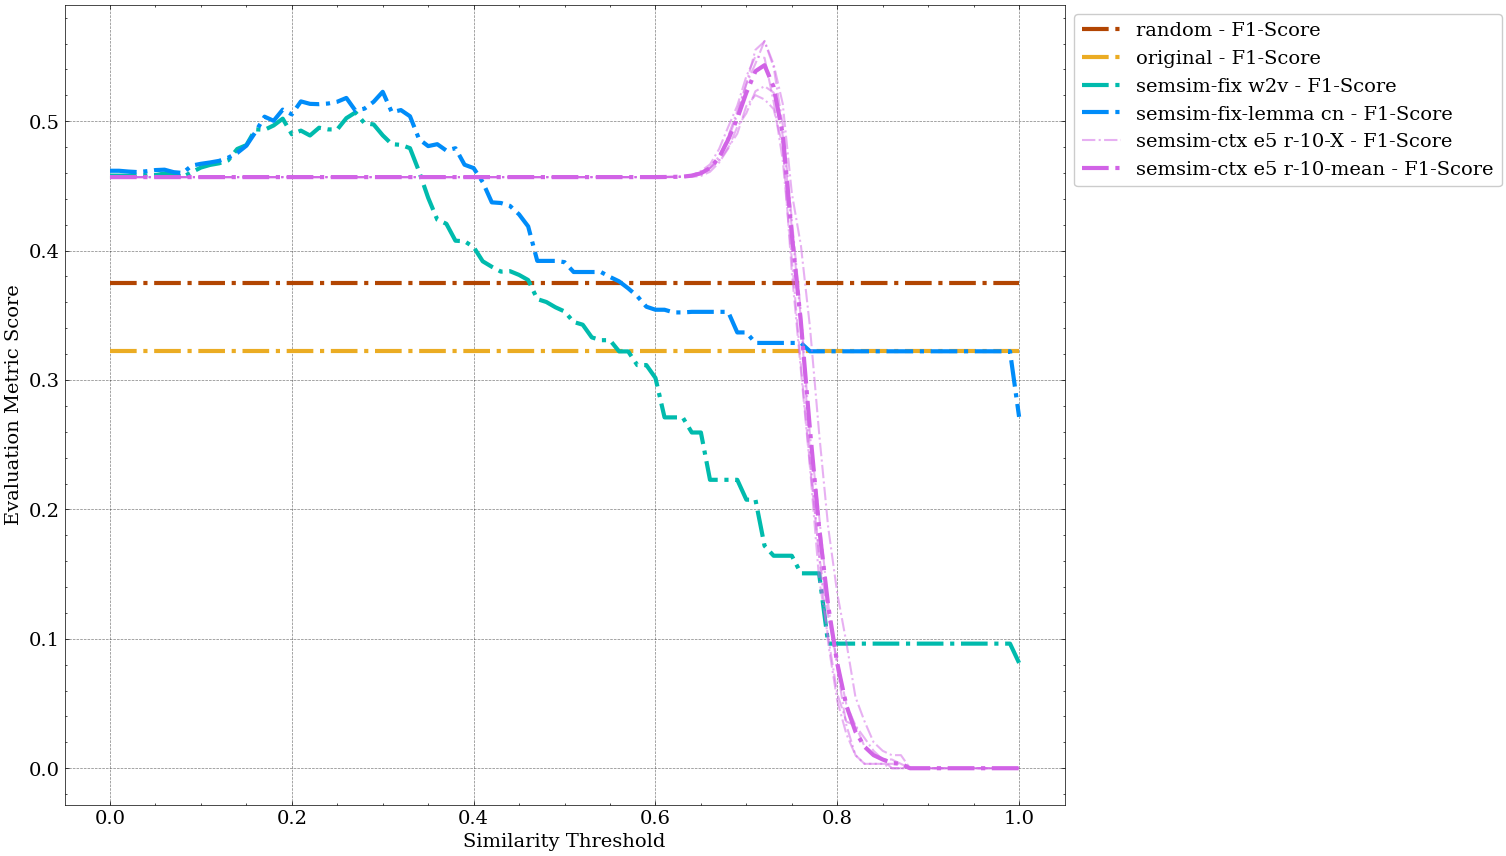
\includegraphics[width=\textwidth]{dataset_conflicts_1-2_pred_wildcard_subsample-2000_evaluation_original_vs_semsim-fix_w2v_vs_semsim-fix-lemma_cn_vs_semsim-ctx_nref-10_e5_f1}
	\caption{F1-score vs. ST for the evaluation runs \texttt{random}, \texttt{original}, \texttt{semsim-fix w2v}, \texttt{semsim-fix-lemma cn} and \texttt{semsim-ctx e5 r-10-X}}
	\label{fig:best-f1-per-pattern}
 \end{subfigure}
 \newline
 \newline
 \begin{subfigure}{\textwidth}
	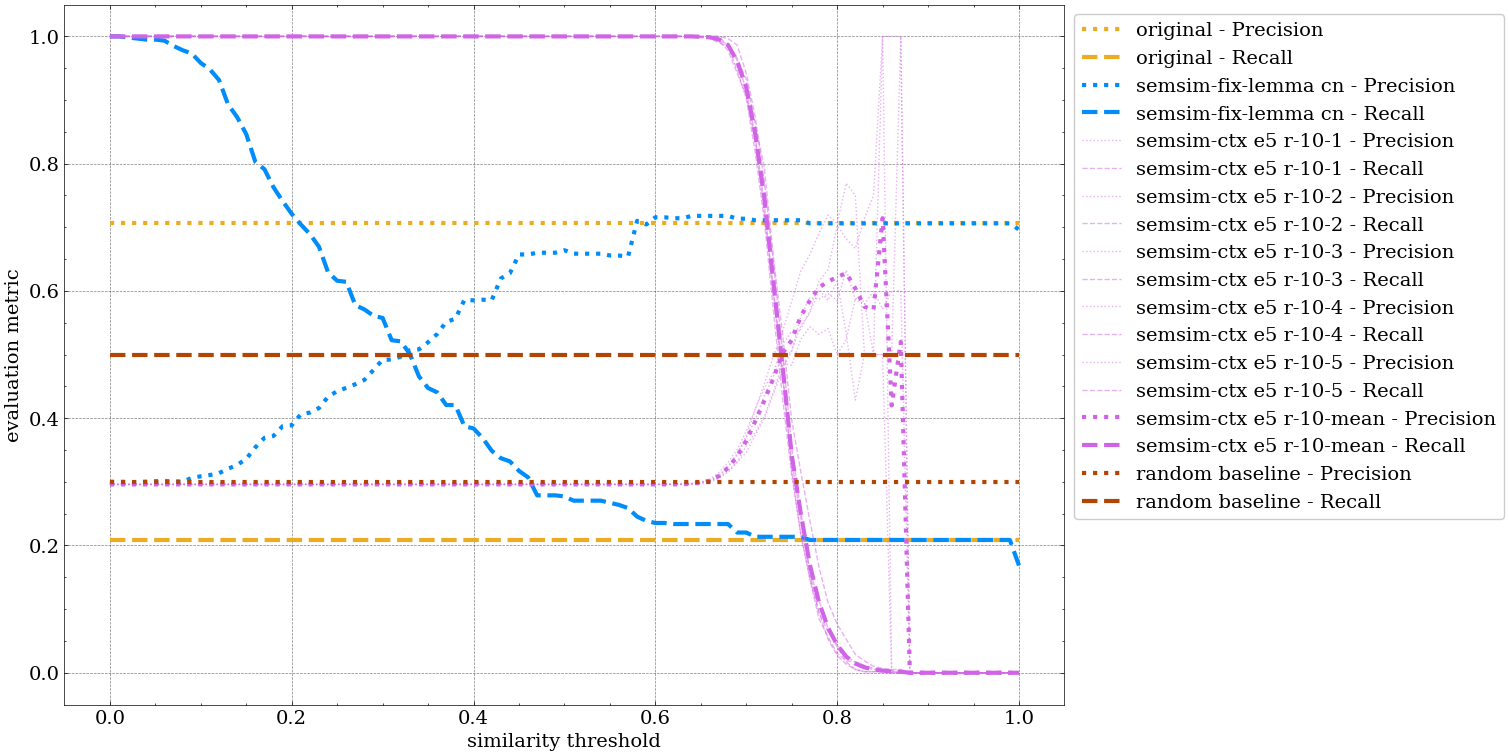
\includegraphics[width=\textwidth]{dataset_conflicts_1-2_pred_wildcard_subsample-2000_evaluation_original_vs_semsim-fix-lemma_cn_vs_semsim-ctx_nref-10_e5_precision-recall}
	\caption{Precision and  recall vs. ST for the evaluation runs \texttt{random}, \texttt{original}, \texttt{semsim-fix-lemma cn} and \texttt{semsim-ctx e5 r-10-X}}
	\label{fig:prec-rec-best-semsim}
 \end{subfigure}
 \caption{Evaluation metric scores vs. similarity threshold values}
\end{figure}
 
%\begin{figure}[hp]
%\centering
%\includegraphics[width=\textwidth]
%%\includegraphics[width=0.85\paperwidth, center]
%{dataset_conflicts_1-2_pred_wildcard_subsample-2000_evaluation_original_vs_semsim-fix_w2v_vs_semsim-fix-lemma_cn_vs_semsim-ctx_nref-10_e5_f1}
%\caption{F1-score vs. ST for the best performing evaluation run configuration for each conflict pattern (including the original pattern)}
%\label{fig:best-f1-per-pattern}
%\end{figure}
%
%\begin{figure}[hp]
%\centering
%%\includegraphics[width=\textwidth]
%\includegraphics[width=\textwidth]
%{dataset_conflicts_1-2_pred_wildcard_subsample-2000_evaluation_original_vs_semsim-fix-lemma_cn_vs_semsim-ctx_nref-10_e5_precision-recall}
%\caption{Precision and  recall vs. ST for the evaluation runs \texttt{original}, \texttt{semsim-fix-lemma cn} and \texttt{semsim-ctx e5 r-10-X}}
%\label{fig:prec-rec-best-semsim}
%\end{figure}


%\begin{figure}
%\centering
%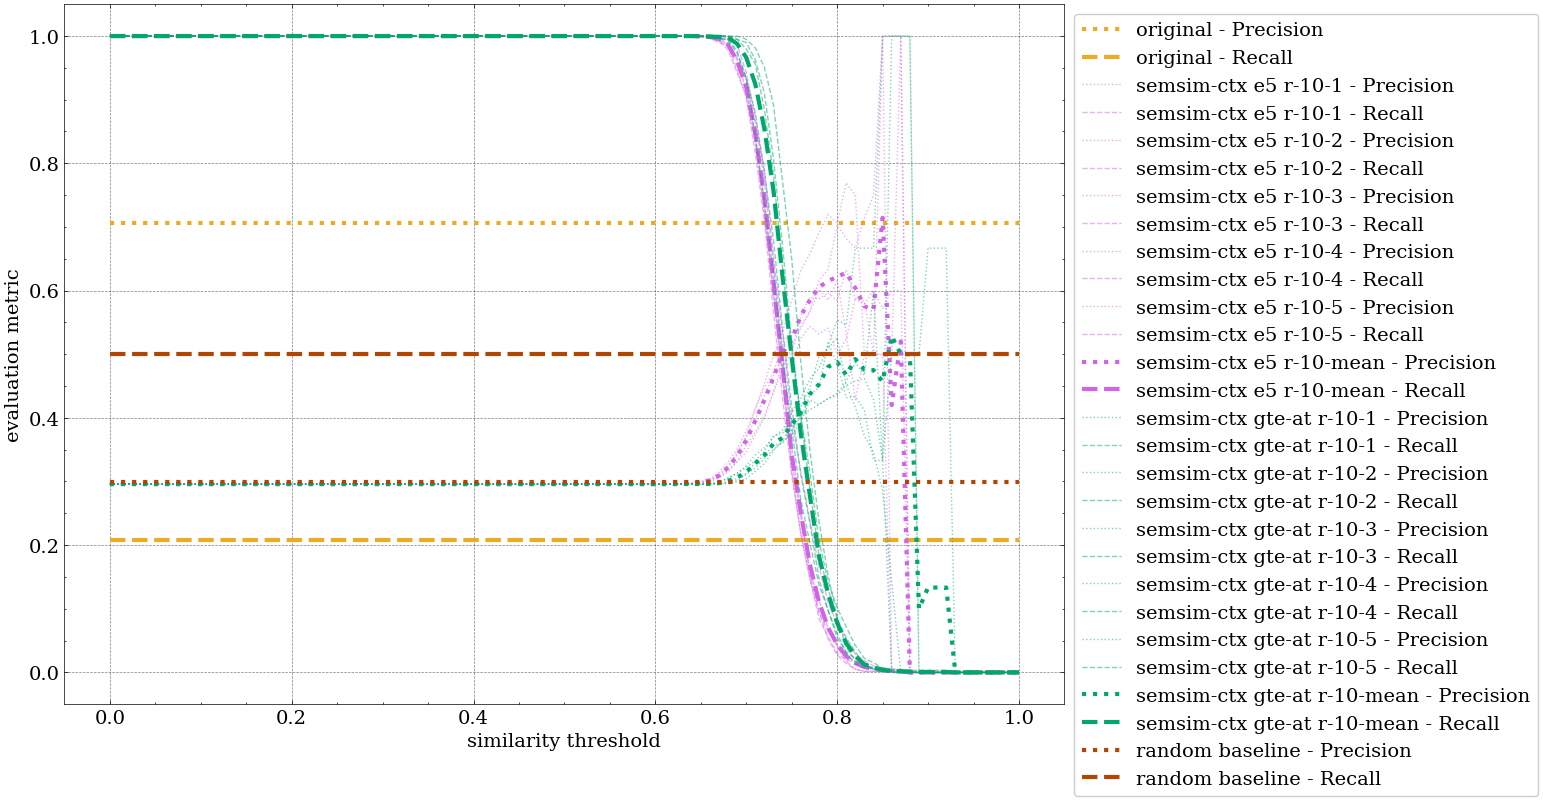
\includegraphics[width=\textwidth]{dataset_conflicts_1-2_pred_wildcard_subsample-2000_evaluation_original_vs_semsim-ctx_nref-10_e5_vs_gte-at_precision-recall}
%\caption{Caption for this figure}
%\label{fig:unique-label-2}
%\end{figure}


\subsection{Best F1-Score vs. Number of Reference Edges}
\label{sec:best-f1-vs-nref}
\Cref{fig:best-f1-vs-nref} visualises the relation of the number of reference edges and the best-F1 score. For this purpose the number of reference edges \texttt{N} is plotted versus the mean RES best F1-score for all ERSs of the form \texttt{semsim-ctx NM-AT r-N-*}.  The standard deviation of the best F1 scores for these ERSs is visualised by the shaded areas around the curves of the mean RES best F1-scores.

\begin{figure}
\centering
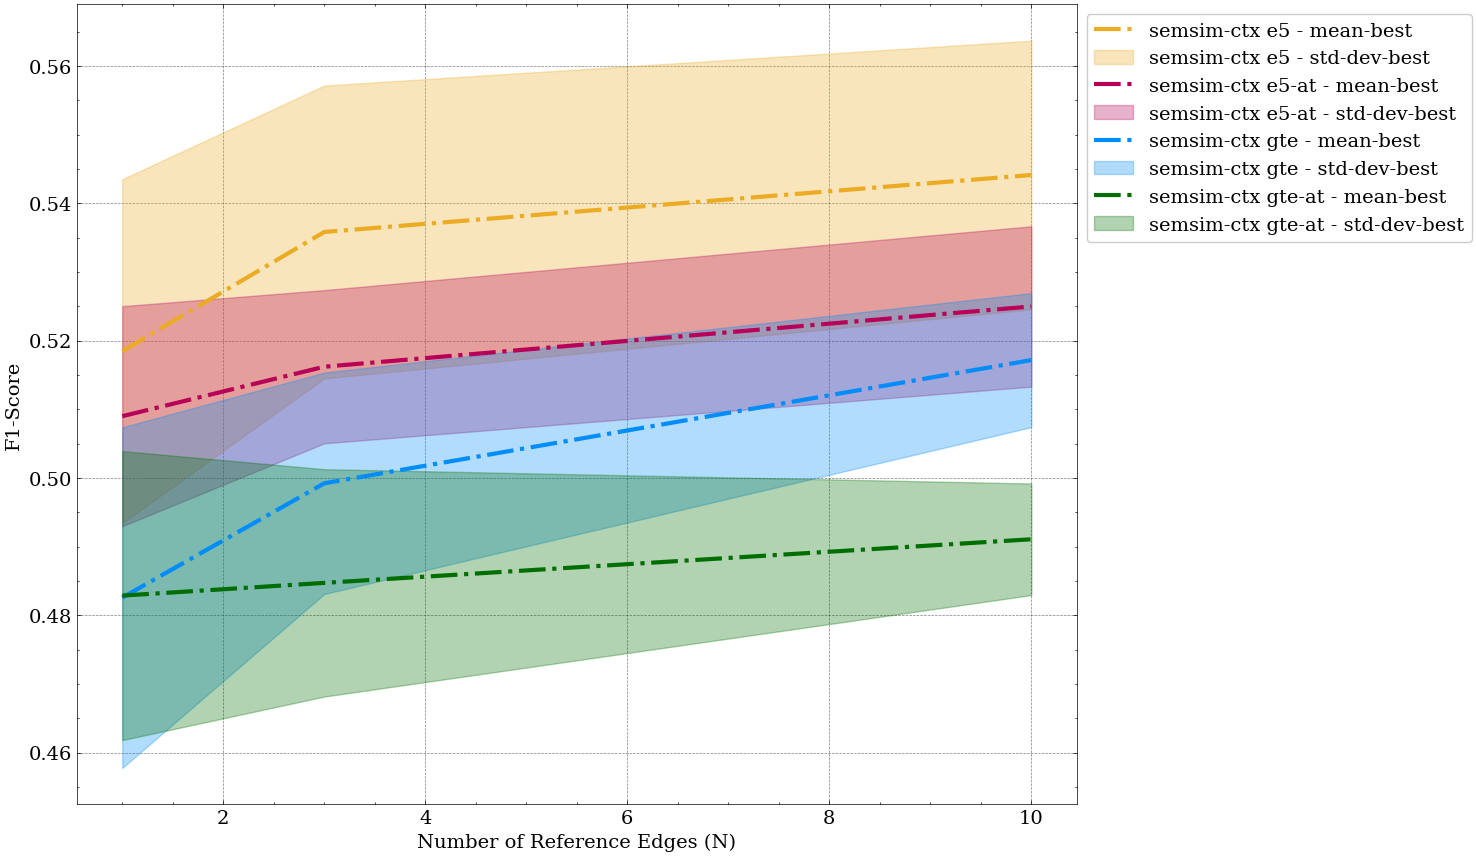
\includegraphics[width=\textwidth]
{/dataset_n_ref_edges/dataset_conflicts_1-2_pred_wildcard_subsample-2000_best-f1_nref_vs_f1}
\caption{Mean reference edge set best F1-score for the ERSs \texttt{semsim-ctx e5 r-N-*}, \texttt{semsim-ctx e5-at r-N-*}, \texttt{semsim-ctx gte-at r-N-*} and \texttt{semsim-ctx gte-at r-N-*}}
\label{fig:best-f1-vs-nref}
\end{figure}

\subsubsection{Significant Observations}
\begin{enumerate}[label=\arabic{listcounter}.\arabic*]
\refstepcounter{listcounter}% Increment the list counter
	\item The mean RES best F1-score of the evaluation runs in an ERS of the form \texttt{semsim-ctx NM(-AT) r-\(N_1\)-*} is higher than the mean RES best F1-score of the evaluation runs in an ERS of the form \texttt{semsim-ctx NM(-AT) r-\(N_2\)-*}, if \(N_2 > N_1\) for \(N_1, N_2 \in \{1, 3, 10\}\) \label{obs-itm:CNESS-more-refs-higher-mean-best-f1}
	\item The standard deviation of the mean RES best F1-score of the evaluation runs in an ERS of the form \texttt{semsim-ctx NM(-AT) r-\(N_1\)-*} is lower than the standard deviation of the mean RES best F1-score of the evaluation runs in an ERS of the form \texttt{semsim-ctx NM(-AT) r-\(N_2\)-*}, if \(N_2 > N_1\) for \(N_1, N_2 \in \{1, 3, 10\}\), except for \texttt{semsim-ctx et-at r-3-*} (\(sd_1 = 0.11\)) and \texttt{semsim-ctx et-at r-10-*} (\(sd_2 = 0.12\)) \label{obs-itm:CNESS-more-refs-lower-stddev-best-f1}
%	\item , where \(sd_2 > sd_2\)
\end{enumerate}



\subsection{Predicate Lemma based Evaluation Run Comparison}
In this section it is explored how the different NESS systems differ in which edges they match. This is done by following up on the concept of the predicate lemma introduced in \cref{sec:base-edge-set}. In \cref{sec:dataset-characteristics} one of the two desired characteristics of the dataset states that it should contain the largest possible number of edges per unique predicate lemma. Specifically it is of interest, how the CNESS system performs in comparison to the FNESS system for subsets of edges which share the same predicate lemma. Such a subset of edges of the conflict dataset is in the following referred to as \textit{predicate lemma edge set} (PLES).


%\subsubsection{Evaluation Runs Representing the NESS System Types}
\paragraph{NESS Type Representatives}
Two evaluation runs are selected to represent the two versions of the NESS systems for the comparison. The lemma-based version of FNESS is chosen here, because of its superior performance regarding best F1-score that is observed in \cref{sec:best-f1-score-eval-run-comparison} and \cref{sec:eval-metrics-vs-st}. Specifically, the evaluation runs \texttt{semsim-fix-lemma cn t-0.30} (evaluation run \textit{A}) and \texttt{semsim-ctx e5 r-10-2 t-0.72} (evaluation run \textit{B}) are selected as representatives of the FNESS and CNESS system respectively. These are the best performing evaluation runs regarding F1-score for the respective semsim conflict patterns (i.e. NESS system), which can be seen in \cref{tab:best-f1-score-mean-best} and \cref{tab:best-f1-score-mean-best-semsim-ctx}.\footnote{
The latter table specifically shows that the evaluation runs \texttt{semsim-ctx e5 r-1-2 t-0.67}, \texttt{semsim-ctx e5 r-10-2 t-0.72} and \texttt{semsim-ctx e5 r-10-4 t-0.72} all correspond to an F1 score \(s_\text{F1} = 0.56\). The evaluation runs utilizing the RESs of size \(N = 10\) are chosen over the one utilizing an RES of size \(N = 1\), because of their generally superior performance regarding F1 score, which is observed in \cref{sec:best-f1-vs-nref}. Among the two remaining evaluation runs, \texttt{semsim-ctx e5 r-10-2 t-0.72} is selected randomly.


%While the lemma-based FNESS system is only able to match all or none of the edges in a PLES, the CNESS system is potentially able to differentiate between "conflict" and "no conflict" given a PLES.
%It shall be noted there that the FNESS system is able to differentiate between different verb forms forms corresponding to the same lemma, when using the semsim-fix and not the semsim-fix-lemma functional pattern. Nonetheless this is assumed to add relevant semantic differentiation capabilities to the FNESS system based on the observed 

}

\subsubsection{PLES Evaluation Score based Evaluation Run Comparison}

\paragraph{Label Balance Ratio}
The \textit{label balance ratio} (LBR) measures how balanced the labels in a given set of labelled edges are. It is calculated by \cref{eq:label-balance-ratio}. Here \(n_\text{pos}\) and \(n_\text{neg}\) are the number of positively ("conflict") and negatively ("no conflict") labeled edges in the edge set.
An edge set with fully balanced labels has \(LBR = 1\) and completely unbalanced labeled edge set has \(LBR = 0\).

\begin{equation}
LBR = 1 - \left(\frac{\left|n_{\text{pos}} - n_{\text{neg}}\right|}{n_{\text{pos}} + n_{\text{neg}}}\right)
\label{eq:label-balance-ratio}
\end{equation}

The evaluation metrics are computed for evaluation run A and B for each PLES, along with metrics that measure distributional properties of a PLES. Namely the number of edges \(n_e\), the number of positively labeled and negatively labeled edges (\(n_\text{pos}\) and \(n_\text{neg}\)), the LBR  and the entropy of a PLES.

\Cref{tab:predicate-lemma-highest-f1} lists the ten predicate lemmas for whose PLES the absolute difference in F1-score, which is achieved in the two evaluation runs, is the highest. Conversely \cref{tab:predicate-lemma-lowest-f1} lists the ten predicate lemma for whose PLES the difference in F1-score which is achieved in the tow evaluation runs is the lowest. In both tables the predicate lemmas have been filtered beforehand, so that only PLES with \(n_s >= 5\) samples are considered. Additionally the recalls (\(r_A, r_B\)) achieved by both evaluation runs regarding a PLES must fulfil the condition that \(r_A + r_B > 0\), i.e. at least the recall achieved by one of the evaluation runs must be non-zero. \Cref{tab:predicate-lemma-highest-f1-both-recall-non-zero} follows the same concept as \cref{tab:predicate-lemma-highest-f1}, except for the condition regarding the recalls being \(r_A * r_B > 0\), i.e. both recalls achieved by the tow evaluation runs must be non-zero. This second variant of the table is not shown for \cref{tab:predicate-lemma-lowest-f1}, because it only lists lemmas for whose PLES the F1-score achieved by both evaluation runs is zero.

\todo[inline]{should I add a table with the actual labels produced by the evaluation runs?}
%An comparison of the actual labels that were produced  by evaluation runs A and B for all PLES corresponding to the lemmas in \cref{tab:predicate-lemma-highest-precision} can be found in \cref{app-sec:ples-eval-labels}.
%specifically in \cref{tab:ples-labels-1}, \cref{tab:ples-labels-2}, \cref{tab:ples-labels-3}, \cref{tab:ples-labels-4}, \cref{tab:ples-labels-5}, \cref{tab:ples-labels-6} and \cref{tab:ples-labels-7} 

%\Cref{tab:predicate-lemma-f1} lists the ten predicate lemmas for whose PLES the best F1-scores are achieved in both of the two evaluation runs.

%\begin{table}[hp]
%\centering
%\begin{tabular}{lrr|lrr}
%\toprule
%\multicolumn{3}{c|}{\texttt{semsim-fix-lemma cn} at \(t_s = 0.30\)} & \multicolumn{3}{c}{\texttt{semsim-ctx e5 r-10-2} at \(t_s = 0.72\)} \\ 
%\midrule
%Lemma      & F1-score & Num. of Samples & Lemma      & F1-score & Num. of Samples \\
%\midrule
%arrest     & 1.00     & 11            & arrest     & 1.00     & 11            \\
%accuse     & 0.97     & 33            & file       & 1.00     & 5             \\
%warn       & 0.93     & 24            & attack     & 1.00     & 12            \\
%slam       & 0.92     & 7             & accuse     & 0.95     & 33            \\
%attack     & 0.91     & 12            & slam       & 0.92     & 7             \\
%criticize  & 0.91     & 6             & criticize  & 0.91     & 6             \\
%detain     & 0.89     & 5             & shoot      & 0.89     & 5             \\
%shoot      & 0.89     & 5             & order      & 0.88     & 14            \\
%condemn    & 0.84     & 25            & detain     & 0.86     & 5             \\
%dismiss    & 0.80     & 6             & launch     & 0.86     & 14            \\ 
%\bottomrule
%\end{tabular}
%\caption{Top ten lemmas regarding F1-score with number of samples per lemma \(n_s >= 5\) \\
%for the evaluation runs \texttt{semsim-fix-lemma cn t-0.30} and \texttt{semsim-ctx e5 r-10-2 t-0.72}}
%\label{tab:predicate-lemma-f1}
%\end{table}
%

\begin{table}[p]
\centering
\begin{tabular}{lccccccc}
\toprule
Lemma      & F1 Diff. & F1 A & F1 B & \(n_e\) & \(n_\text{pos}\)/\(n_\text{neg}\) & LBR & Entropy \\
\midrule
file       & 1.00      & 0.00           & 1.00           & 5               & 5/0     & 0.00 & 0.00 \\
order      & 0.88      & 0.00           & 0.88           & 14              & 7/7     & 1.00 & 1.00 \\
launch     & 0.86      & 0.00           & 0.86           & 14              & 8/6     & 0.86 & 0.99 \\
step       & 0.80      & 0.00           & 0.80           & 5               & 2/3     & 0.80 & 0.97 \\
target     & 0.77      & 0.00           & 0.77           & 8               & 6/2     & 0.50 & 0.81 \\
use        & 0.75      & 0.00           & 0.75           & 14              & 5/9     & 0.71 & 0.94 \\
block      & 0.73      & 0.00           & 0.73           & 8               & 4/4     & 1.00 & 1.00 \\
take       & 0.71      & 0.00           & 0.71           & 19              & 6/13    & 0.63 & 0.90 \\
open       & 0.67      & 0.00           & 0.67           & 8               & 1/7     & 0.25 & 0.54 \\
suspend    & 0.67      & 0.00           & 0.67           & 6               & 2/4     & 0.67 & 0.92 \\
build      & 0.67      & 0.00           & 0.67           & 6               & 1/5     & 0.33 & 0.65 \\
\cmidrule{7-8}
\multicolumn{6}{l}{} & \multicolumn{2}{c}{mean} \\
\multicolumn{6}{l}{} & 0.61 & 0.79 \\
\bottomrule
\end{tabular}
\caption{Top ten lemmas regarding the highest difference in F1-score between the evaluation runs with recalls \(r_A + r_B > 0\) and number of samples per lemma \(n_s >= 5\) for the evaluation runs \texttt{semsim-fix-lemma cn t-0.30} (A) and \texttt{semsim-ctx e5 r-10-2 t-0.72} (B)}
\label{tab:predicate-lemma-highest-f1}
\end{table}

\begin{table}[p]
\centering
\begin{tabular}{lccccccc}
\toprule
Lemma      & F1 Diff. & F1 A & F1 B & \(n_e\) & \(n_\text{pos}\)/\(n_\text{neg}\) & LBR & Entropy \\
\midrule
accept     & 0.42      & 0.25           & 0.67           & 7               & 1/6     & 0.29 & 0.59 \\
strike     & 0.30      & 0.80           & 0.50           & 9               & 6/3     & 0.67 & 0.92 \\
capture    & 0.22      & 0.44           & 0.67           & 7               & 2/5     & 0.57 & 0.86 \\
seize      & 0.17      & 0.67           & 0.50           & 12              & 6/6     & 1.00 & 1.00 \\
deny       & 0.17      & 0.50           & 0.67           & 6               & 2/4     & 0.67 & 0.92 \\
suggest    & 0.17      & 0.33           & 0.50           & 5               & 1/4     & 0.40 & 0.72 \\
warn       & 0.12      & 0.93           & 0.81           & 24              & 21/3    & 0.25 & 0.54 \\
claim      & 0.12      & 0.43           & 0.55           & 22              & 6/16    & 0.55 & 0.85 \\
attack     & 0.09      & 0.91           & 1.00           & 12              & 10/2    & 0.33 & 0.65 \\
threaten   & 0.09      & 0.52           & 0.61           & 20              & 7/13    & 0.70 & 0.93 \\
approve    & 0.08      & 0.12           & 0.20           & 16              & 1/15    & 0.12 & 0.34 \\
\cmidrule{7-8}
\multicolumn{6}{l}{} & \multicolumn{2}{c}{mean} \\
\multicolumn{6}{l}{} & 0.50 & 0.76 \\
\bottomrule
\end{tabular}
\caption{Top ten lemmas regarding the highest difference in F1-score between the evaluation runs with recalls \(r_A \cdot r_B > 0\) and number of samples per lemma \(n_s >= 5\) for the evaluation runs \texttt{semsim-fix-lemma cn t-0.30} (A) and \texttt{semsim-ctx e5 r-10-2 t-0.72} (B)}
\label{tab:predicate-lemma-highest-f1-both-recall-non-zero}
\end{table}


\begin{table}[htp]
\centering
\begin{tabular}{lccccccc}
\toprule
Lemma      & F1 Diff. & F1 A & F1 B & \(n_e\) & \(n_\text{pos}\)/\(n_\text{neg}\) & LBR & Entropy \\
\midrule
arrest     & 0.00      & 1.00           & 1.00           & 11              & 11/0    & 0.00 & 0.00 \\
slam       & 0.00      & 0.92           & 0.92           & 7               & 6/1     & 0.29 & 0.59 \\
criticize  & 0.00      & 0.91           & 0.91           & 6               & 5/1     & 0.33 & 0.65 \\
shoot      & 0.00      & 0.89           & 0.89           & 5               & 4/1     & 0.40 & 0.72 \\
condemn    & 0.00      & 0.84           & 0.84           & 25              & 18/7    & 0.56 & 0.86 \\
dismiss    & 0.00      & 0.80           & 0.80           & 6               & 4/2     & 0.67 & 0.92 \\
tell       & 0.01      & 0.49           & 0.50           & 28              & 9/19    & 0.64 & 0.91 \\
accuse     & 0.02      & 0.97           & 0.95           & 33              & 31/2    & 0.12 & 0.33 \\
kill       & 0.02      & 0.66           & 0.64           & 77              & 38/39   & 0.99 & 1.00 \\
say        & 0.03      & 0.45           & 0.48           & 31              & 9/22    & 0.58 & 0.87 \\
\cmidrule{7-8}
\multicolumn{6}{l}{} & \multicolumn{2}{c}{mean} \\
\multicolumn{6}{l}{} & 0.46 & 0.68 \\
\bottomrule
\end{tabular}
\caption{Top ten lemmas regarding the lowest absolute difference in F1-score between the evaluation runs with recalls \(r_A + r_B > 0\) and number of samples per lemma \(n_s >= 5\) for the evaluation runs \texttt{semsim-fix-lemma cn t-0.30} (A) and \texttt{semsim-ctx e5 r-10-2 t-0.72} (B)}
\label{tab:predicate-lemma-lowest-f1}
\end{table}

\subsubsection{Significant Observations}
\begin{enumerate}[label=\arabic{listcounter}.\arabic*]
\refstepcounter{listcounter}% Increment the list counter
	\item The CNESS utilizing evaluation run achieves a higher F1-score than the FNESS utilizing evaluation run for every PLES of the the top ten PLES regarding highest difference in F1-score between the two evaluation runs (independently of the recall condition) \label{obs-itm:CNESS-higher-f1-for-highest-f1-difference}
	\item The mean LBR and mean entropy of the top ten PLESs regarding the highest difference in F1-score between the two evaluation runs are higher than the mean LBR and mean entropy of the top ten PLESs regarding the lowest difference in F1-score between the two evaluation runs (independently of the recall condition) \label{obs-itm:PLES-more-diverse-for-highest-f1-difference}
	\item The differences in F1-score achieved by the two evaluation runs is higher for the recall condition \(r_A + r_B > 0\) than for \(r_A \cdot r_B > 0\), because for the first condition the F1-score of the FNESS evaluation run is zero for all PLESs \label{obs-itm:FNESS-zero-recall-highest-f1-difference}
	\item The lemmas corresponding to the the top ten PLES regarding highest difference in F1-score between the two evaluation runs are all not included in the conflict verbs: "accuse", "arrest", "clash", "condemn", "kill", "slam" \label{obs-itm:conflict-verbs-not-in-highest-f1-difference}
	\item Of the lemmas corresponding to  the top ten PLES regarding lowest difference in F1-score between the two evaluation runs, five of six are included in the conflict verbs: "arrest", "condemn", "kill", "slam" ("clash" is not included) \label{obs-itm:conflict-verbs-in-lowest-f1-difference}
%	\item Of the lemmas corresponding the to the the top ten PLES regarding highest difference in F1-score given the recall condition \(r_A + r_B > 0\), most are intuitively not considered to clearly relate to the definition of conflict
%	\item Of the lemmas corresponding the to  the top ten PLES regarding highest difference in F1-score given the recall condition \(r_A \cdot r_B > 0\) and of the lemmas corresponding the to the top ten PLES regarding lowest difference in F1-score, most are intuitively considered to clearly relate to the definition of conflict


\end{enumerate}


\section{Result Discussion}
\label{sec:result-discussion}
In this section the previously presented evaluation results are discussed. It synthesizes the major insights derived from the observations of the different result data perspectives. The discussion is organized into categories and sub-categories, which relate to the research questions outlined in \cref{sec:research-questions}. Here retrieval performance generally refers to joined measure of precision and recall and therefore means F1-score, as stated above in \cref{sec:evaluation-metrics}. 


\subsection{Retrieval Performance Improvement}

\begin{itemize}

\item NESS-SHMP can achieve a better retrieval performance than the original conflict pattern, independent of NESS type and configuration (depending on the ST) \\
\textbf{Supporting Observations:} \Cref{obs-itm:NESS-higher-best-f1}

\item CNESS-SHPM using the sub tokens embedding can achieve the overall best retrieval performance (in comparison to FNESS-SHMP and the original conflict pattern) \\
\textbf{Supporting Observations:} \Cref{obs-itm:NESS-higher-best-f1}, \Cref{obs-itm:CNESS-higher-best-f1-than-FNESS}

\item Using lemma-based FNESS-SHMP instead of word-based FNESS-SHMP can achieve a better retrieval performance \\
\textbf{Supporting Observations:} \Cref{obs-itm:lemma-based-FNESS-higher-best-f1}, \Cref{obs-itm:lemma-FNESS-higher-f1-nearly-always}

\end{itemize}


\subsubsection{Similarity Threshold Impact}

\begin{itemize}

\item The relation of ST and NESS-SHMP retrieval performance and therefore the relevant ST range depends primarily on the NESS type \\
\textbf{Supporting Observations:} \Cref{obs-itm:ASTR-lemma-FNESS-cn-higher-than-CNESS-e5} \Cref{obs-itm:ASTR-FNESS-higher-than-CNESS} \Cref{obs-itm:ASTR-FNESS-equal}

\item The relation of ST and CNESS-SHMP retrieval performance depends secondarily on the NESS model and the usage of the all tokens option \\
\textbf{Supporting Observations:} \Cref{obs-itm:ASTR-CNESS-gte-starts-earlier} \Cref{obs-itm:ASTR-CNESS-at-starts-earlier} \Cref{obs-itm:ASTR-CNESS-end-equal}

\end{itemize}


\subsubsection{NESS Configuration Impact}

\begin{itemize}

\item Using a generally better performing NESS model (regarding established benchmarks) does not generally improve the NESS-SHMP retrieval performance \\
\textbf{Supporting Observations:} \Cref{obs-itm:lemma-FNESS-cn-better-than-w2v}, \Cref{obs-itm:word-FNESS-w2v-better-than-cn}, \Cref{obs-itm:CNESS-e5-better-than-gte}

\item Using the sub tokens embedding instead of the all tokens embedding improves retrieval performance, but using the all tokens embedding makes it less sensible to the selection of the reference edges
\\ \textbf{Supporting Observations:} \Cref{obs-itm:CNESS-better-without-AT}, \Cref{obs-itm:CNESS-lower-variation-with-AT}

\item CNESS-SHPM retrieval performance improves with a higher number of reference edges and is less sensible to the specific selection of reference edges
\\ \textbf{Supporting Observations:} \Cref{obs-itm:CNESS-more-refs-higher-mean-best-f1}, \Cref{obs-itm:CNESS-more-refs-lower-stddev-best-f1}

\end{itemize}


\subsection{Retrieval Precision Behaviour}

\begin{itemize}
	\item The precision of NESS-SHMPM correlates with the ST until a specific value of the ST, which itself is specific to the NESS type, NESS model (and other CNESS parameters, especially the selection of reference edges)
\\ \textbf{Supporting Observations:} \Cref{obs-itm:FNESS-ST-precision-correlates}, \Cref{obs-itm:CNESS-ST-precision-correlates-until-crosspoint}, \Cref{obs-itm:FNESS-ST-limit}

\item CNESS-SHMP achieves on average the same precision as the original conflict pattern and lemma-based FNESS, although CNESS-SHMP can achieve a higher precision, it depends on the selection of the reference edges \\
\textbf{Supporting Observations:} \Cref{obs-itm:CNESS-precision-variation-higher-ASTR}, \Cref{obs-itm:CNESS-highest-precision-equal-original}


\end{itemize}

\subsection{Contextual Differentiation Ability}

\begin{itemize}
	\item CNESS-SHPM is able differentiate when matching a set of edges where purely symbolic SHPM and FNESS-SHMPM cannot, i.e. cases where context is needed to determine the correct semantics of word \\
	\textbf{Supporting Observations:} \Cref{obs-itm:CNESS-higher-f1-for-highest-f1-difference}, \Cref{obs-itm:PLES-more-diverse-for-highest-f1-difference}, \Cref{obs-itm:conflict-verbs-not-in-highest-f1-difference}, \Cref{obs-itm:conflict-verbs-in-lowest-f1-difference}
	
	\item While CNESS-SHPM achieves a highest difference in retrieval performance for sets of edges, where FNESS-SHMP does not match, it also achieves a better retrieval performance in cases where FNESS-SHPM does match \\
	\textbf{Supporting Observations:} \Cref{obs-itm:CNESS-higher-f1-for-highest-f1-difference} \Cref{obs-itm:FNESS-zero-recall-highest-f1-difference}
		
\end{itemize}

\todo[inline]{Add or integrate more direct answer to the research questions}








% ========== 
\chapter{Conclusion}

\chapter{Future Work}
\section{Conceptual Improvements}
Somehow extend the token span used for CNESS beyond the word tokens but not to all tokens. Use the tokens of the next best sub-edge e.g. although in the case of a predicate this is probably the entire sentence most of the time.

\section{Implementation Improvements}
implemnt multiprocessing, i.e. server process for both hypergraph and semsim matchers. 

other option would be to leverage python shared memory capabilities but is likely to be less stable and has less scaling potential

\section{Further Evaluations}


\printbibliography
\appendix
\chapter{Appendix}
\section{Reference Edge Sets}
\label{app-sec:ref-edge-sets}

\begin{table}[H]
\begin{tabular}{cc p{10cm}}
\toprule
\multicolumn{1}{c}{Num. of}			& \multicolumn{1}{c}{Ref. Edges}		& \multicolumn{1}{l}{Reference Edge Content} \\
\multicolumn{1}{c}{Ref. Edges}		& \multicolumn{1}{c}{Set ID}			& \multicolumn{1}{c}{} \\
\midrule
1 & 1-1 & Israeli gunfire wounds Gaza fisherman: ministry \\
\hline
1 & 1-2 & Ukraine’s Opposition Accuses Government of Provoking Violence \\
\hline
1 & 1-3 & Thursday's attack by armed youths on the base in Bor left at least 58 dead, including children \\
\hline
1 & 1-4 & Turkey suspends 15,200 education staff \\
\hline
1 & 1-5 & Kurdish protesters storm the Conservative Party's campaign headquarters in London \\
\hline
3 & 3-1 & Israeli gunfire wounds Gaza fisherman: ministry \\
 &  & Kuwait Rejects Saudi Request for War Subvention \\
 &  & Researchers Accuse Canadian Internet Company of Helping Yemen Censor the Web \\
\hline
3 & 3-2 & Ukraine’s Opposition Accuses Government of Provoking Violence \\
 &  & Chinese island-building in the South China Sea is causing "irreversible and widespread damage to biodiversity and ecological balance," according to the Philippines; Manila accused China of disregarding the people who rely on the sea by destroying coral reefs to create new islands \\
 &  & The government's opposition and various refugee organizations have harshly criticized the reforms \\
\hline
3 & 3-3 & Thursday's attack by armed youths on the base in Bor left at least 58 dead, including children \\
 &  & Venezuela expels 3 US consular officials \\
 &  & Russia, China nix U.S. human rights claims: Russia and China disputed U.S. Ambassador Nikki Haley's contention that human rights violations are a main driver of conflicts \\
\hline
3 & 3-4 & Turkey suspends 15,200 education staff \\
 &  & Leading Muslim groups condemn ISIS killing of US journalists \\
 &  & PayPal freezes Canadian media company's account over story about Syrian family \\
\hline
3 & 3-5 & Kurdish protesters storm the Conservative Party's campaign headquarters in London \\
 &  & Obama seeks new Syria strategy review to deal with ISIS \\
 &  & Tougher Canadian visa policy hits foreign workers, protects Canadian jobs \\
\bottomrule
\end{tabular}
\caption{Edge content for the reference edge sets of size \(N \in \{1, 3\}\)}
\label{tab:ref-edge-sets-nref-1-3}
\end{table}

\begin{table}[H]
\begin{tabular}{cc p{10cm}}
\toprule
\multicolumn{1}{c}{Num. of}			& \multicolumn{1}{c}{Ref. Edges}		& \multicolumn{1}{l}{Reference Edge Content} \\
\multicolumn{1}{c}{Ref. Edges}		& \multicolumn{1}{c}{Set ID}			& \multicolumn{1}{c}{} \\
\midrule
10 & 10-1 & Israeli gunfire wounds Gaza fisherman: ministry \\
 &  & Kuwait Rejects Saudi Request for War Subvention \\
 &  & Researchers Accuse Canadian Internet Company of Helping Yemen Censor the Web \\
 &  & Afghanistan President Ashraf Ghani slams Pakistan for harbouring terrorists, praises India \\
 &  & 5-year-old Kentucky boy fatally shoots 2-year-old sister \\
 &  & Bangladesh police kill 'mastermind' of Dhaka cafe attack \\
 &  & Philippines President Duterte orders army to destroy Islamic militants or risk ISIS disease \\
 &  & Turkish jets kill 18 Daesh terrorists in northern Syria \\
 &  & Report slams Israel's military law enforcement system \\
 &  & Iran Pursuing Release of Sailors Abducted by Somalian Pirates \\
\hline
10 & 10-2 & Ukraine’s Opposition Accuses Government of Provoking Violence \\
 &  & Chinese island-building in the South China Sea is causing "irreversible and widespread damage to biodiversity and ecological balance," according to the Philippines; Manila accused China of disregarding the people who rely on the sea by destroying coral reefs to create new islands \\
 &  & The government's opposition and various refugee organizations have harshly criticized the reforms \\
 &  & Syria and Russia oppose unilateral US strikes against ISIL in Syria \\
 &  & Taliban attack in Afghanistan kills six policemen \\
 &  & Turkish President condemns US commandos photographed sporting Kurdish militia insignia \\
 &  & France could ease ban on gay men giving blood after ECJ ruling \\
 &  & Libyan smuggler fighting kills 22 migrants \\
 &  & Kazakhstan jails online editor for 'spreading false information \\
 &  & Russia urges Assad to give up chemical weapons \\
\bottomrule
\end{tabular}
\caption{Edge content for the reference edge sets of size \(N = 10\) (Part 1/3)}
\label{tab:ref-edge-sets-nref-10-part-1}
\end{table}

\begin{table}[H]
\begin{tabular}{cc p{10cm}}
\toprule
\multicolumn{1}{c}{Num. of}			& \multicolumn{1}{c}{Ref. Edges}		& \multicolumn{1}{l}{Reference Edge Content} \\
\multicolumn{1}{c}{Ref. Edges}		& \multicolumn{1}{c}{Set ID}			& \multicolumn{1}{c}{} \\
\midrule
10 & 10-3 & Thursday's attack by armed youths on the base in Bor left at least 58 dead, including children \\
 &  & Venezuela expels 3 US consular officials \\
 &  & Russia, China nix U.S. human rights claims: Russia and China disputed U.S. Ambassador Nikki Haley's contention that human rights violations are a main driver of conflicts \\
 &  & Turkish PM tells female reporter to 'know your place \\
 &  & South Korean prosecutors seek arrest of ex-President Park in corruption probe \\
 &  & Taliban Announce Spring Offensive in Afghanistan \\
 &  & Spain dismantles 'jihadist cell \\
 &  & U.S. conducts 'counter terrorism strike' against al Qaeda-linked target in Libya \\
 &  & Swiss prosecutors launch money-laundering probe against fugitive Ukrainian President Yanukovych, and son \\
 &  & UK Wants 10 Year Prison Sentence For Online Pirates \\
\hline
10 & 10-4 & Turkey suspends 15,200 education staff \\
 &  & Leading Muslim groups condemn ISIS killing of US journalists \\
 &  & PayPal freezes Canadian media company's account over story about Syrian family \\
 &  & U.S. urges China's Xi to extend non-militarization pledge to all of South China Sea \\
 &  & Sri Lanka accuses Canada of holding Commonwealth 'to ransom \\
 &  & Russia and pro-Moscow rebels on Wednesday condemned Ukraine for ratifying two bills on greater autonomy for the separatist east, saying they violated a peace deal and threatened a shaky month-long truce \\
 &  & Malaysia turns away 800 boat people; Thailand spots 3rd boat \\
 &  & US expresses concern over security of Pakistan’s Nuclear weapons \\
 &  & Health experts accuse WHO of ‘egregious failure’ on Ebola \\
 &  & Sunni militants accuse the army, perhaps the only widely respected public institution in Lebanon, of siding with Hezbollah \\
\bottomrule
\end{tabular}
\caption{Edge content for the reference edge sets of size \(N = 10\) (Part 2/3)}
\label{tab:ref-edge-sets-nref-10-part-2}
\end{table}


\begin{table}[H]
\begin{tabular}{cc p{10cm}}
\toprule
\multicolumn{1}{c}{Num. of}			& \multicolumn{1}{c}{Ref. Edges}		& \multicolumn{1}{l}{Reference Edge Content} \\
\multicolumn{1}{c}{Ref. Edges}		& \multicolumn{1}{c}{Set ID}			& \multicolumn{1}{c}{} \\
\midrule
10 & 10-5 & Kurdish protesters storm the Conservative Party's campaign headquarters in London \\
 &  & Obama seeks new Syria strategy review to deal with ISIS \\
 &  & Tougher Canadian visa policy hits foreign workers, protects Canadian jobs \\
 &  & U.S. preparing new sanctions against Chinese entities over financial support to North Korea \\
 &  & Turkey's Erdogan makes Nazi jibe over Germany rally ban: "Your practices are not different from the Nazi practices of the past \\
 &  & Brazil committee recommends Dilma Rousseff's impeachment \\
 &  & U.S. dismisses Russian concern about missile defense system in South Korea \\
 &  & South Korea mulls ban on bosses messaging employees at home \\
 &  & Israel to destroy homes of Palestinian Jerusalem car attackers \\
 &  & Majority of Finns reject NATO membership \\
\bottomrule
\end{tabular}
\caption{Edge content for the reference edge sets of size \(N = 10\) (Part 3/3)}
\label{tab:ref-edge-sets-nref-10-part-3}
\end{table}

\section{Best F1-score based Eval. Run Comparison Tables}
\label{app-sec:result-tables}

\begin{table}[H]
\centering
\begin{tabular}{lllrrrrrr}
\toprule
\multicolumn{4}{l}{Evaluation Run Name} & \multicolumn{1}{c}{Prec.} & \multicolumn{1}{c}{Rec.} & \multicolumn{2}{c}{(Best) F1-Score}\\
\cmidrule{1-4}\cmidrule{7-8}
\multicolumn{1}{l}{CP} & \multicolumn{1}{l}{NM} & \multicolumn{1}{l}{RES} & \multicolumn{1}{c}{\(t_s\)} & \multicolumn{3}{l}{} & \multicolumn{1}{c}{Std. Dev.} \\
\midrule
semsim-ctx & e5 & r-1-1 & 0.65 & 0.386 & 0.768 & 0.514 & - \\
semsim-ctx & e5 & r-1-2 & 0.67 & 0.442 & 0.769 & 0.562 & - \\
semsim-ctx & e5 & r-1-3 & 0.59 & 0.372 & 0.838 & 0.515 & - \\
semsim-ctx & e5 & r-1-4 & 0.67 & 0.363 & 0.804 & 0.500 & - \\
semsim-ctx & e5 & r-1-5 & 0.68 & 0.397 & 0.681 & 0.502 & - \\
semsim-ctx & e5 & r-1-mean & 0.64 & 0.356 & 0.823 & 0.477 & +/- 0.046 \\
semsim-ctx & e5 & r-1-mean-best & 0.65 & 0.392 & 0.772 & 0.518 & +/- 0.025 \\
\hline
semsim-ctx & e5 & r-3-1 & 0.68 & 0.398 & 0.836 & 0.539 & - \\
semsim-ctx & e5 & r-3-2 & 0.68 & 0.435 & 0.752 & 0.551 & - \\
semsim-ctx & e5 & r-3-3 & 0.69 & 0.410 & 0.846 & 0.553 & - \\
semsim-ctx & e5 & r-3-4 & 0.69 & 0.392 & 0.846 & 0.536 & - \\
semsim-ctx & e5 & r-3-5 & 0.68 & 0.361 & 0.814 & 0.500 & - \\
semsim-ctx & e5 & r-3-mean & 0.69 & 0.417 & 0.753 & 0.534 & +/- 0.024 \\
semsim-ctx & e5 & r-3-mean-best & 0.68 & 0.399 & 0.818 & 0.536 & +/- 0.021 \\
\hline
semsim-ctx & e5 & r-10-1 & 0.71 & 0.415 & 0.817 & 0.550 & - \\
semsim-ctx & e5 & r-10-2 & 0.72 & 0.435 & 0.793 & 0.562 & - \\
semsim-ctx & e5 & r-10-3 & 0.72 & 0.400 & 0.771 & 0.527 & - \\
semsim-ctx & e5 & r-10-4 & 0.72 & 0.454 & 0.735 & 0.562 & - \\
semsim-ctx & e5 & r-10-5 & 0.71 & 0.378 & 0.835 & 0.520 & - \\
semsim-ctx & e5 & r-10-mean & 0.72 & 0.428 & 0.746 & 0.543 & +/- 0.021 \\
semsim-ctx & e5 & r-10-mean-best & 0.72 & 0.416 & 0.790 & 0.544 & +/- 0.020 \\
\hline
semsim-ctx & gte & r-1-1 & 0.60 & 0.349 & 0.794 & 0.485 & - \\
semsim-ctx & gte & r-1-2 & 0.63 & 0.388 & 0.799 & 0.522 & - \\
semsim-ctx & gte & r-1-3 & 0.57 & 0.303 & 0.972 & 0.462 & - \\
semsim-ctx & gte & r-1-4 & 0.55 & 0.300 & 1.000 & 0.461 & - \\
semsim-ctx & gte & r-1-5 & 0.61 & 0.339 & 0.829 & 0.482 & - \\
semsim-ctx & gte & r-1-mean & 0.60 & 0.327 & 0.870 & 0.474 & +/- 0.013 \\
semsim-ctx & gte & r-1-mean-best & 0.59 & 0.336 & 0.879 & 0.483 & +/- 0.025 \\
\hline
semsim-ctx & gte & r-3-1 & 0.64 & 0.364 & 0.826 & 0.505 & - \\
semsim-ctx & gte & r-3-2 & 0.67 & 0.378 & 0.713 & 0.494 & - \\
semsim-ctx & gte & r-3-3 & 0.67 & 0.385 & 0.740 & 0.506 & - \\
semsim-ctx & gte & r-3-4 & 0.66 & 0.376 & 0.820 & 0.516 & - \\
semsim-ctx & gte & r-3-5 & 0.62 & 0.322 & 0.896 & 0.474 & - \\
semsim-ctx & gte & r-3-mean & 0.66 & 0.374 & 0.714 & 0.486 & +/- 0.040 \\
semsim-ctx & gte & r-3-mean-best & 0.65 & 0.365 & 0.799 & 0.499 & +/- 0.016 \\
\hline
semsim-ctx & gte & r-10-1 & 0.67 & 0.377 & 0.869 & 0.526 & - \\
semsim-ctx & gte & r-10-2 & 0.67 & 0.361 & 0.917 & 0.518 & - \\
semsim-ctx & gte & r-10-3 & 0.69 & 0.382 & 0.834 & 0.524 & - \\
semsim-ctx & gte & r-10-4 & 0.69 & 0.399 & 0.730 & 0.516 & - \\
semsim-ctx & gte & r-10-5 & 0.68 & 0.388 & 0.708 & 0.501 & - \\
semsim-ctx & gte & r-10-mean & 0.68 & 0.378 & 0.803 & 0.513 & +/- 0.009 \\
semsim-ctx & gte & r-10-mean-best & 0.68 & 0.382 & 0.812 & 0.517 & +/- 0.010 \\
\bottomrule
\end{tabular}
\caption{Best F1-score evaluation runs for all ERS of the form \texttt{semsim-ctx NM r-N-X} (CNESS with AT option disabled)}
\label{tab:best-f1-score-mean-best-semsim-ctx}
\end{table}


\begin{table}[H]
\centering
\begin{tabular}{lllrrrrrr}
\toprule
\multicolumn{4}{l}{Evaluation Run Name} & \multicolumn{1}{c}{Prec.} & \multicolumn{1}{c}{Rec.} & \multicolumn{2}{c}{(Best) F1-Score}\\
\cmidrule{1-4}\cmidrule{7-8}
\multicolumn{1}{l}{CP} & \multicolumn{1}{l}{NM} & \multicolumn{1}{l}{RES} & \multicolumn{1}{c}{\(t_s\)} & \multicolumn{3}{l}{} & \multicolumn{1}{c}{Std. Dev.} \\
\midrule
semsim-ctx & e5-at & r-1-1 & 0.68 & 0.338 & 0.915 & 0.494 & - \\
semsim-ctx & e5-at & r-1-2 & 0.71 & 0.434 & 0.701 & 0.536 & - \\
semsim-ctx & e5-at & r-1-3 & 0.66 & 0.356 & 0.885 & 0.508 & - \\
semsim-ctx & e5-at & r-1-4 & 0.71 & 0.365 & 0.798 & 0.501 & - \\
semsim-ctx & e5-at & r-1-5 & 0.71 & 0.351 & 0.908 & 0.507 & - \\
semsim-ctx & e5-at & r-1-mean & 0.69 & 0.350 & 0.847 & 0.487 & +/- 0.021 \\
semsim-ctx & e5-at & r-1-mean-best & 0.69 & 0.369 & 0.841 & 0.509 & +/- 0.016 \\
\hline
semsim-ctx & e5-at & r-3-1 & 0.72 & 0.363 & 0.846 & 0.508 & - \\
semsim-ctx & e5-at & r-3-2 & 0.72 & 0.389 & 0.765 & 0.516 & - \\
semsim-ctx & e5-at & r-3-3 & 0.73 & 0.399 & 0.780 & 0.528 & - \\
semsim-ctx & e5-at & r-3-4 & 0.73 & 0.386 & 0.829 & 0.526 & - \\
semsim-ctx & e5-at & r-3-5 & 0.72 & 0.351 & 0.886 & 0.503 & - \\
semsim-ctx & e5-at & r-3-mean & 0.73 & 0.392 & 0.740 & 0.511 & +/- 0.016 \\
semsim-ctx & e5-at & r-3-mean-best & 0.72 & 0.378 & 0.821 & 0.516 & +/- 0.011 \\
\hline
semsim-ctx & e5-at & r-10-1 & 0.74 & 0.382 & 0.849 & 0.527 & - \\
semsim-ctx & e5-at & r-10-2 & 0.75 & 0.395 & 0.781 & 0.525 & - \\
semsim-ctx & e5-at & r-10-3 & 0.75 & 0.405 & 0.815 & 0.541 & - \\
semsim-ctx & e5-at & r-10-4 & 0.74 & 0.371 & 0.890 & 0.523 & - \\
semsim-ctx & e5-at & r-10-5 & 0.74 & 0.357 & 0.881 & 0.509 & - \\
semsim-ctx & e5-at & r-10-mean & 0.75 & 0.395 & 0.766 & 0.521 & +/- 0.016 \\
semsim-ctx & e5-at & r-10-mean-best & 0.74 & 0.382 & 0.843 & 0.525 & +/- 0.012 \\
\hline
semsim-ctx & gte-at & r-1-1 & 0.65 & 0.342 & 0.826 & 0.483 & - \\
semsim-ctx & gte-at & r-1-2 & 0.68 & 0.386 & 0.774 & 0.515 & - \\
semsim-ctx & gte-at & r-1-3 & 0.66 & 0.311 & 0.945 & 0.468 & - \\
semsim-ctx & gte-at & r-1-4 & 0.63 & 0.300 & 1.000 & 0.461 & - \\
semsim-ctx & gte-at & r-1-5 & 0.66 & 0.339 & 0.866 & 0.487 & - \\
semsim-ctx & gte-at & r-1-mean & 0.66 & 0.328 & 0.882 & 0.476 & +/- 0.018 \\
semsim-ctx & gte-at & r-1-mean-best & 0.66 & 0.335 & 0.882 & 0.483 & +/- 0.021 \\
\hline
semsim-ctx & gte-at & r-3-1 & 0.69 & 0.340 & 0.827 & 0.482 & - \\
semsim-ctx & gte-at & r-3-2 & 0.69 & 0.309 & 0.950 & 0.467 & - \\
semsim-ctx & gte-at & r-3-3 & 0.72 & 0.348 & 0.852 & 0.494 & - \\
semsim-ctx & gte-at & r-3-4 & 0.71 & 0.367 & 0.822 & 0.508 & - \\
semsim-ctx & gte-at & r-3-5 & 0.67 & 0.317 & 0.930 & 0.473 & - \\
semsim-ctx & gte-at & r-3-mean & 0.69 & 0.324 & 0.883 & 0.472 & +/- 0.013 \\
semsim-ctx & gte-at & r-3-mean-best & 0.70 & 0.336 & 0.876 & 0.485 & +/- 0.017 \\
\hline
semsim-ctx & gte-at & r-10-1 & 0.71 & 0.342 & 0.879 & 0.492 & - \\
semsim-ctx & gte-at & r-10-2 & 0.72 & 0.336 & 0.910 & 0.491 & - \\
semsim-ctx & gte-at & r-10-3 & 0.73 & 0.349 & 0.891 & 0.501 & - \\
semsim-ctx & gte-at & r-10-4 & 0.72 & 0.341 & 0.885 & 0.492 & - \\
semsim-ctx & gte-at & r-10-5 & 0.70 & 0.322 & 0.934 & 0.478 & - \\
semsim-ctx & gte-at & r-10-mean & 0.72 & 0.341 & 0.854 & 0.486 & +/- 0.002 \\
semsim-ctx & gte-at & r-10-mean-best & 0.72 & 0.338 & 0.900 & 0.491 & +/- 0.008 \\\bottomrule
\end{tabular}
\caption{Best F1-score evaluation runs for all ERS of the form \texttt{semsim-ctx NM-at r-N-X} (CNESS with AT option enabled)}
\label{tab:best-f1-score-mean-best-semsim-ctx-at}
\end{table}

\newpage
\section{Evaluation Metric Scores vs. Similarity Threshold Plots}
\label{app-sec:eval-metric-vs-st-plots}

\begin{figure}[H]
\centering
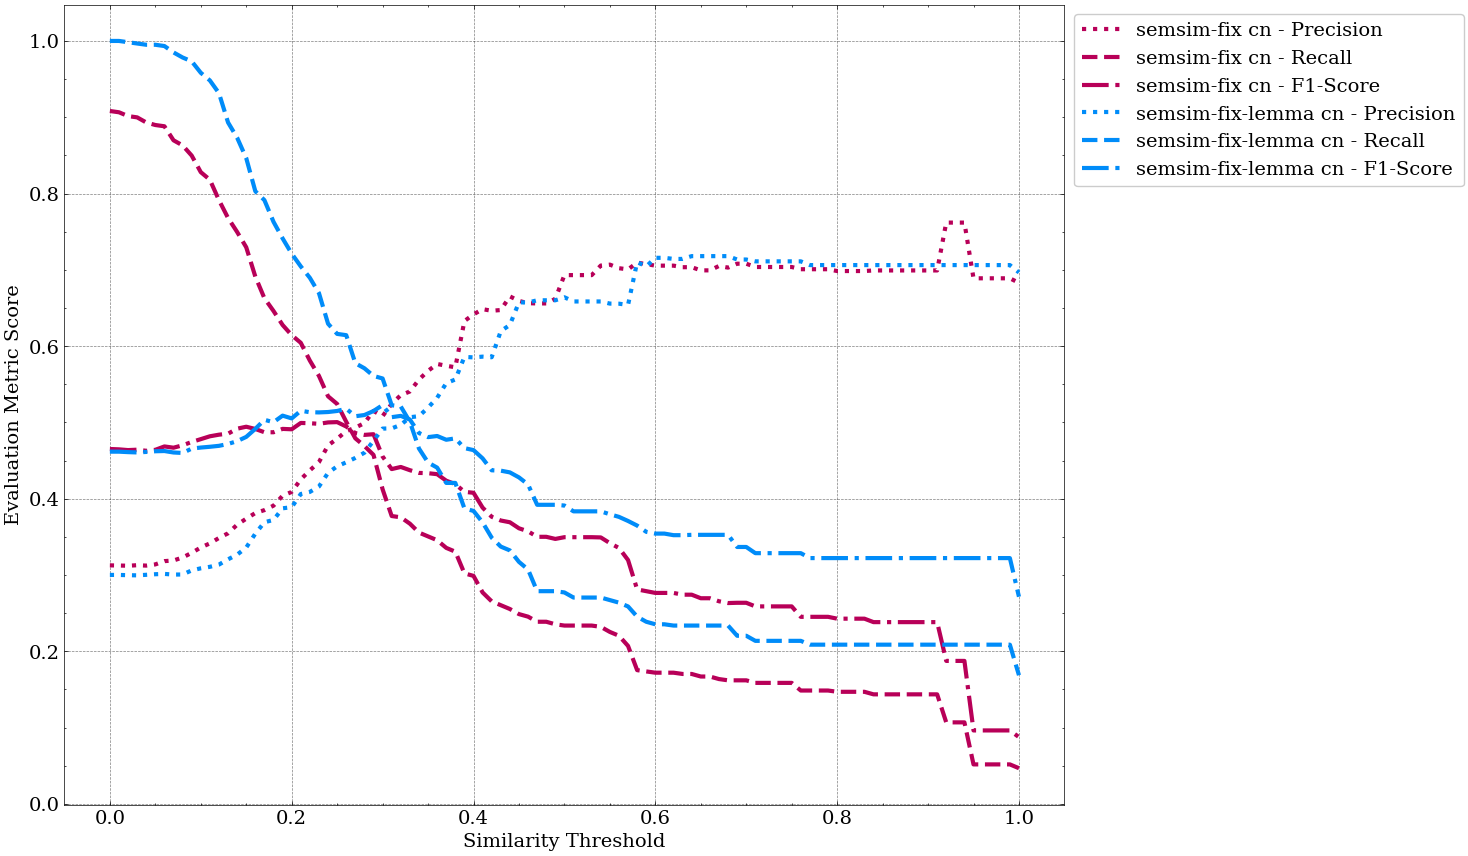
\includegraphics[width=\textwidth]{dataset_conflicts_1-2_pred_wildcard_subsample-2000_evaluation_semsim-fix_cn_vs_semsim-fix-lemma_cn_precision-recall-f1}
\caption{Precision, recall and F1-score vs. ST for the evaluation runs \texttt{semsim-fix cn} and \texttt{semsim-fix-lemma cn}}
\label{fig:prec-rec-f1-semsim-fix-lemma}
\end{figure}

\begin{figure}[H]
\centering
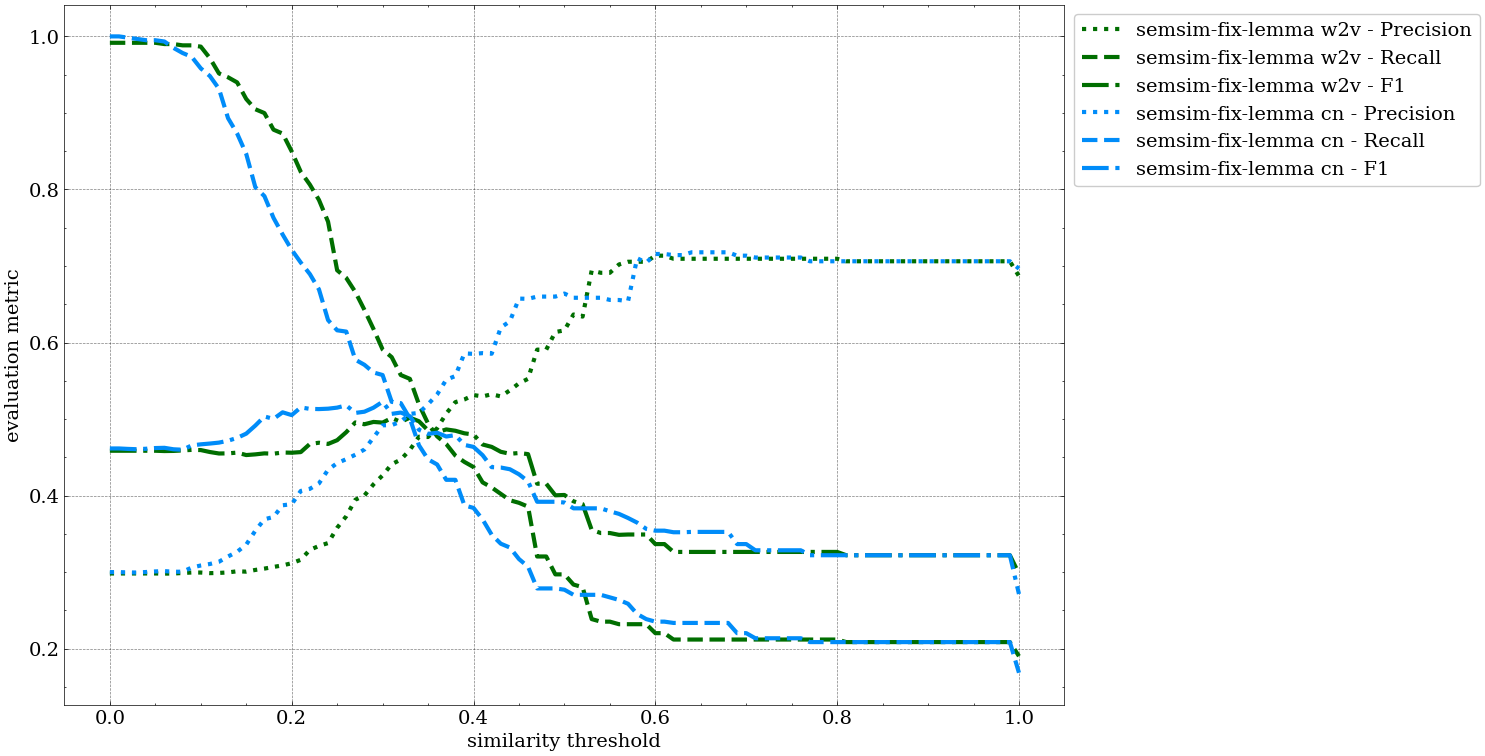
\includegraphics[width=\textwidth]{dataset_conflicts_1-2_pred_wildcard_subsample-2000_evaluation_semsim-fix-lemma_w2v_cn_precision-recall-f1}
\caption{Precision, recall and F1-score vs. ST for the evaluation runs \texttt{semsim-fix-lemma w2v} and \texttt{semsim-fix-lemma cn}}
\label{fig:prec-rec-f1-semxim-fix-lemma-model}
\end{figure}

\begin{figure}[H]
\centering
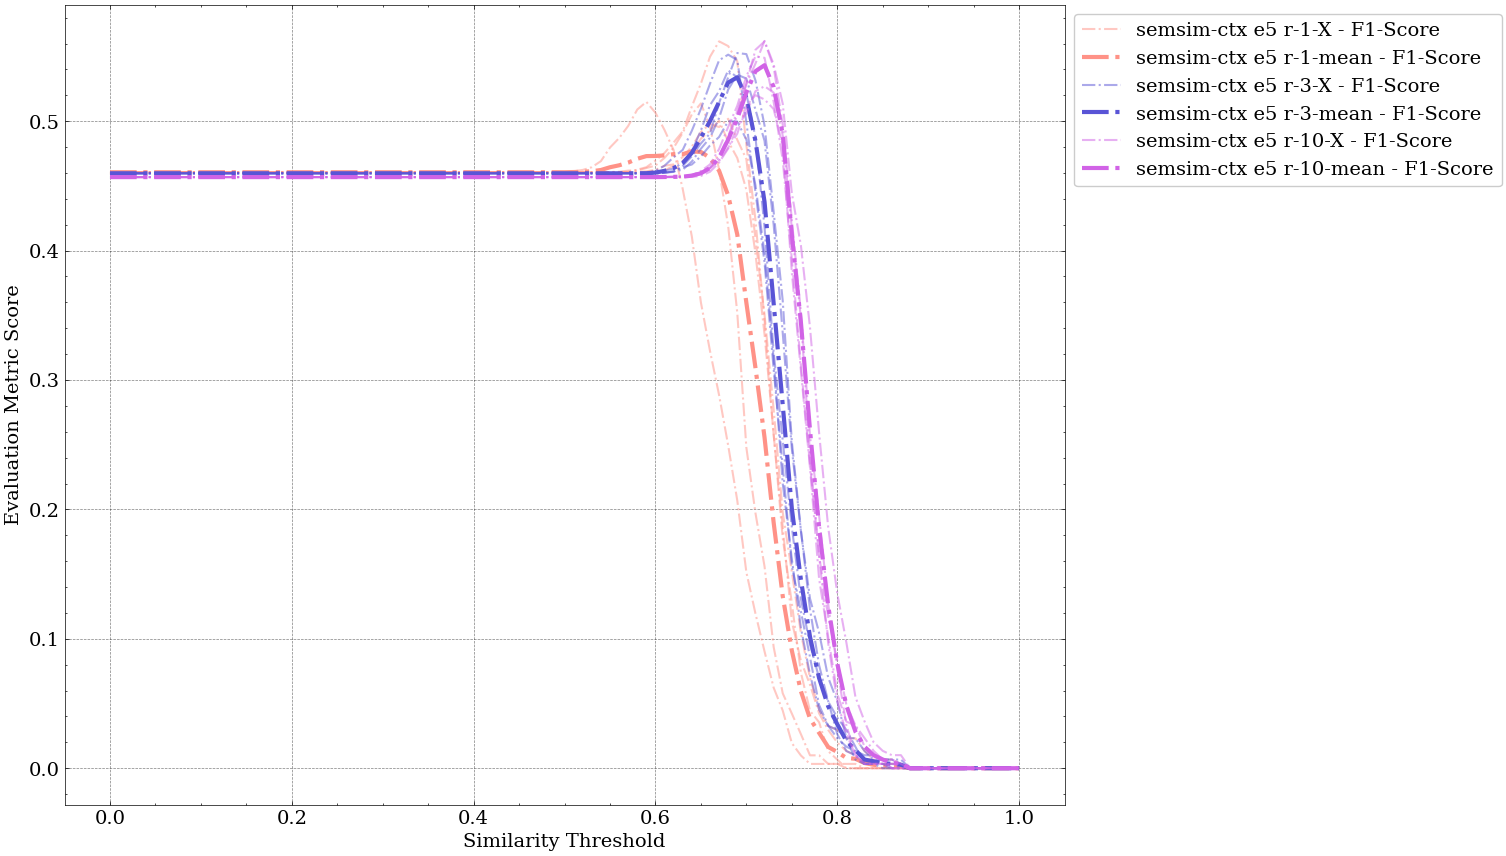
\includegraphics[width=\textwidth]{dataset_conflicts_1-2_pred_wildcard_subsample-2000_evaluation_semsim-ctx_e5_nref-1_vs_nref-3_vs_nref-10_f1}
\caption{F1-score vs. ST for the evaluation runs \texttt{semsim-ctx e5 r-1-X}, \texttt{semsim-ctx e5 r-3-X} and \texttt{semsim-ctx e5 r-10-X}}
\label{fig:f1-semsim-ctx-nref}
\end{figure}

\begin{figure}[H]
\centering
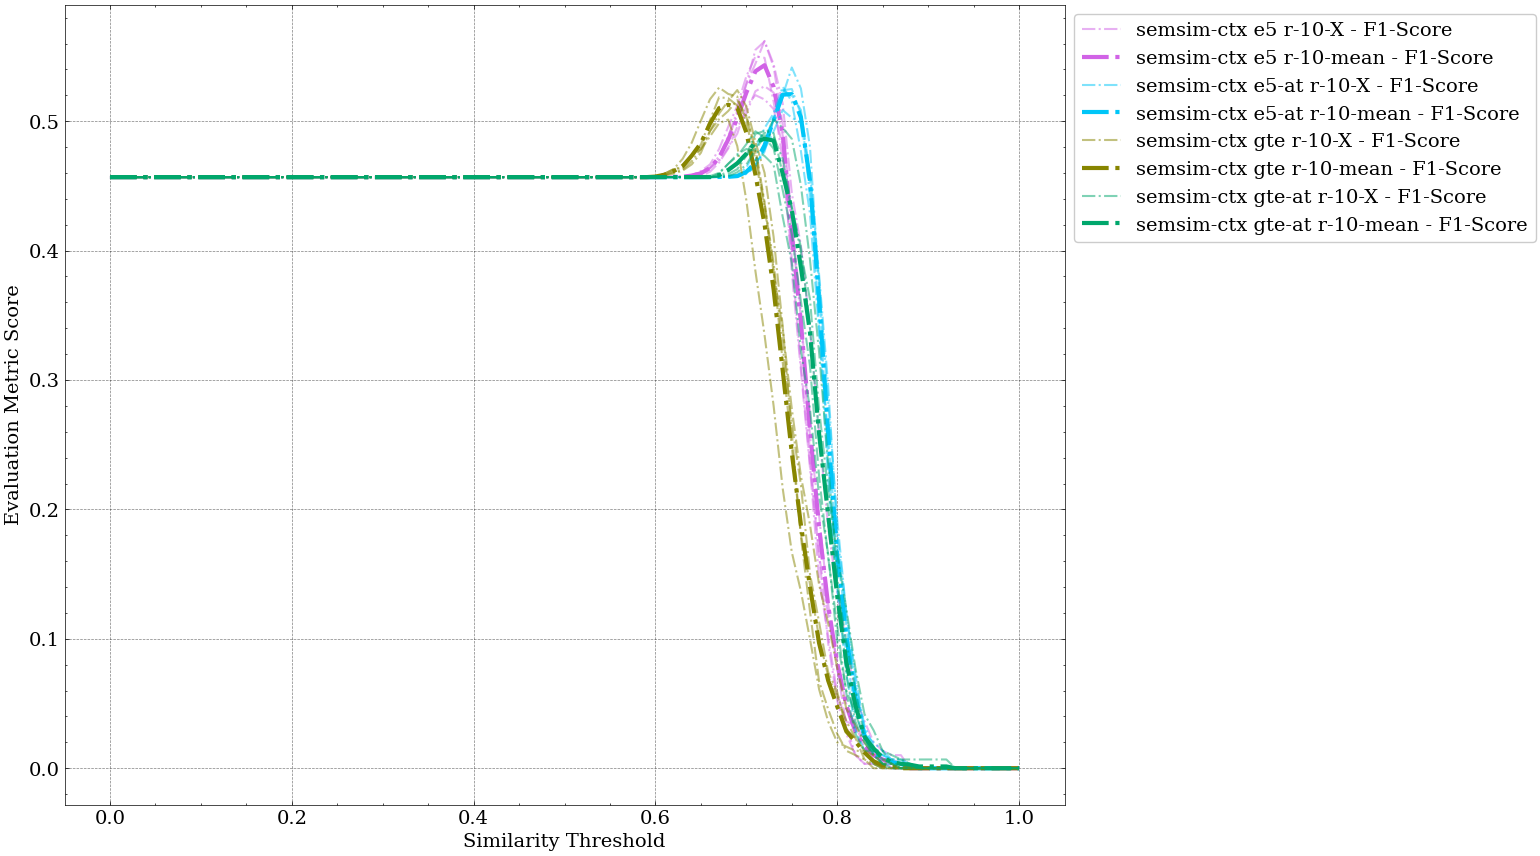
\includegraphics[width=\textwidth]{dataset_conflicts_1-2_pred_wildcard_subsample-2000_evaluation_semsim-ctx_nref-10_e5_e5-at_gte_gte-at_f1}
\caption{F1-score vs. ST for the evaluation runs \texttt{semsim-ctx e5 r-10-X}, \texttt{semsim-ctx e5-at r-10-X}, \texttt{semsim-ctx gte r-10-X} and \texttt{semsim-ctx gte-at r-10-X}}
\label{fig:f1-semsim-ctx-model-at}
\end{figure}

\begin{figure}[H]
\centering
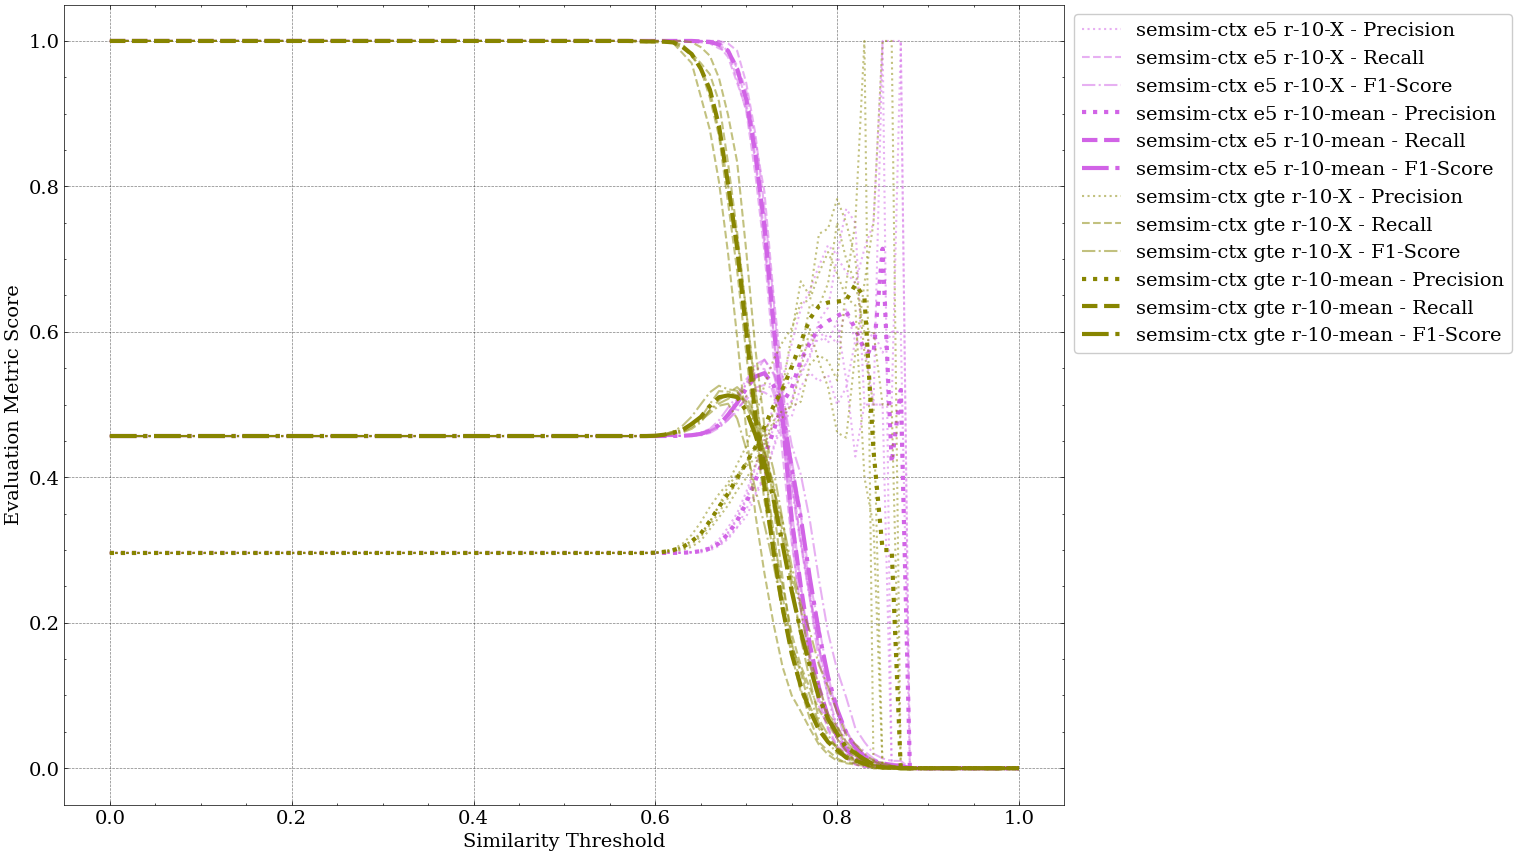
\includegraphics[width=\textwidth]{dataset_conflicts_1-2_pred_wildcard_subsample-2000_evaluation_semsim-ctx_nref-10_e5_vs_gte_precision-recall-f1}
\caption{Precision, recall and F1-score vs. ST for the evaluation runs \texttt{semsim-ctx e5 r-10-X} and \texttt{semsim-ctx gte r-10-X}}
\label{fig:prec-rec-f1-semsim-ctx-model}
\end{figure}

\begin{figure}[H]
\centering
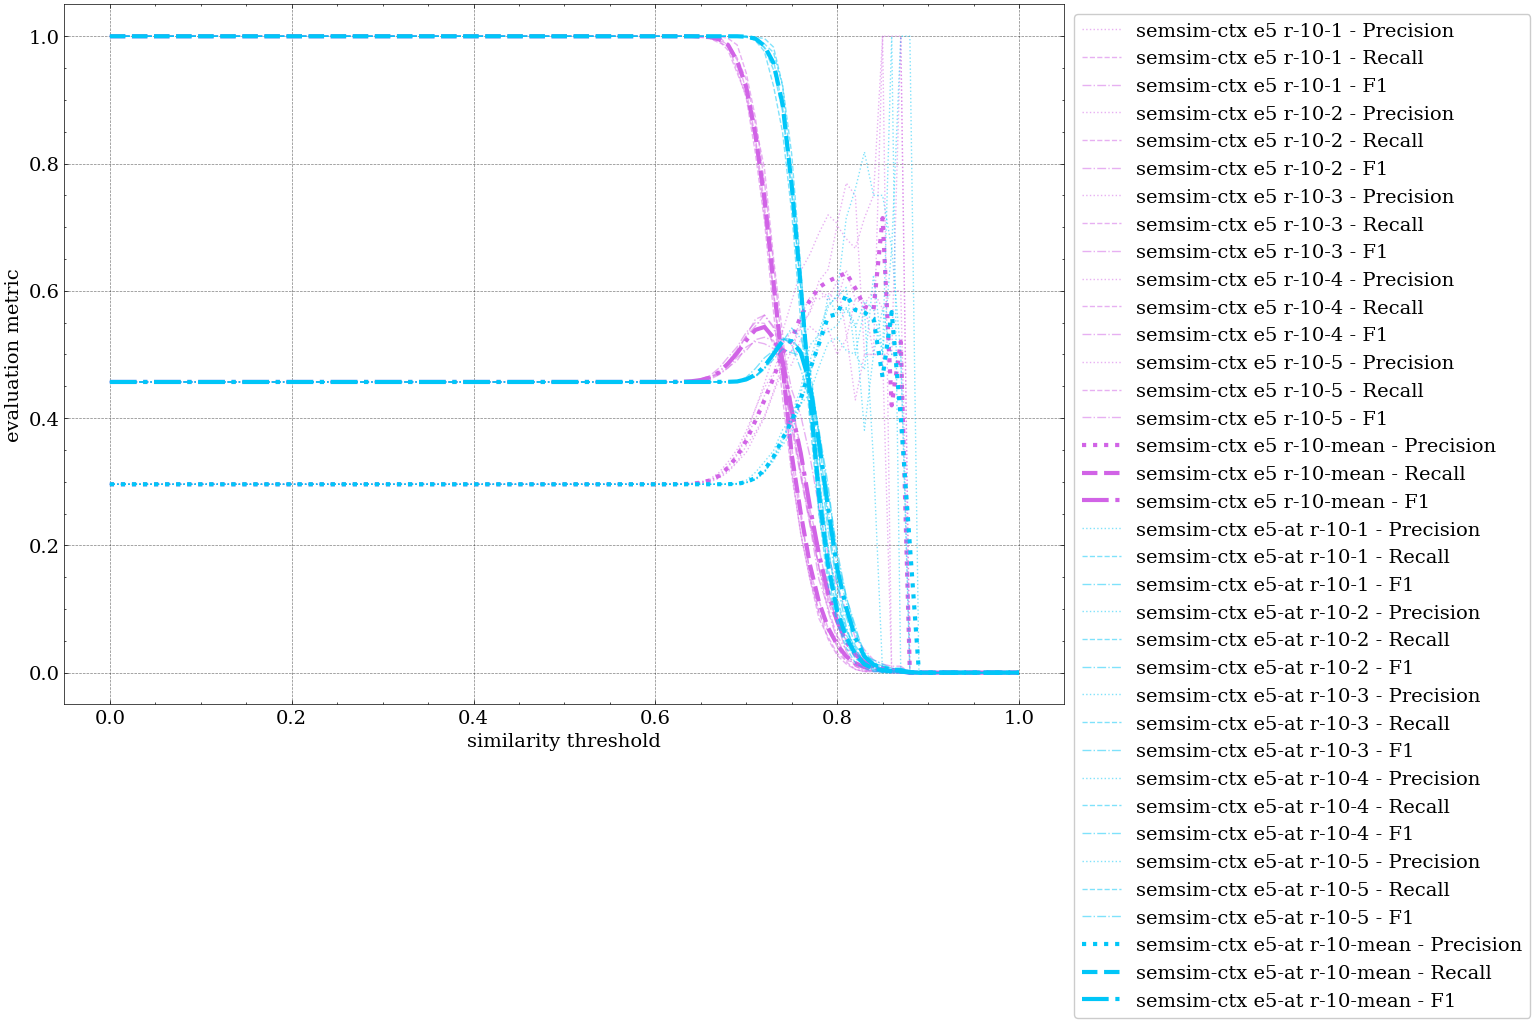
\includegraphics[width=\textwidth]{dataset_conflicts_1-2_pred_wildcard_subsample-2000_evaluation_semsim-ctx_nref-10_e5-vs_e5-at_precision-recall-f1}
\caption{Precision, recall and F1-score vs. ST for the evaluation runs \texttt{semsim-ctx e5 r-10-X} and \texttt{semsim-ctx e5-at r-10-X}}
\label{fig:prec-rec-f1-semsim-ctx-at}
\end{figure}



%\newpage
%\section{PLES Evaluation Label Comparison Tables}
%\label{app-sec:ples-eval-labels}
%
%\begin{sidewaystable}[htp]
%\centering
%\begin{tabular}{l p{13cm} ccc}
%\toprule
%Lemma (\(n\_s\)) & Edge Content & Label Dataset & Label Eval. A & Label Eval. B \\
%\midrule
%capture (7) & Video captures horror of Istanbul airport attack & no conflict & conflict & no conflict) \\
%& Syrian Troops Capture Village Near Northern City of Aleppo & no conflict & conflict & no conflict \\
%& Iraqi forces capture key parts of Mosul neighborhood & no conflict & conflict & no conflict \\
%& Iraqi forces capture west Mosul's main buildings in pre-dawn raid & no conflict & conflict & no conflict \\
%& The videos capture 10 seconds of movement, just enough to catch trucks’ license plates—the operation’s main objective & no conflict & conflict & no conflict \\
%& Security Service of Ukraine Captured Russian Spy & conflict & conflict & conflict \\
%& Syrian Army strikes back in Deir Ezzor: Tal Barouk captured (Report + Video & conflict & conflict & no conflict \\
%\hline
%accept (7)
%& Saudi blogger Badawi's wife accepts Sakharov Prize & no conflict & conflict & no conflict \\
%& UK accepts 1,500 asylum seekers from Syria & no conflict & conflict & no conflict \\
%& Syria rebel chief rejects US-Russia chemical arms deal — “We cannot accept any part of this initiative & conflict & conflict & conflict \\
%& Catholic hospitals accept birth control compromise & no conflict & conflict & conflict \\
%& Japan accepts less than 1\% of asylum applications & no conflict & conflict & no conflict \\
%& Nato accepts Afghan leader Karzai's air strikes decree & no conflict & conflict & no conflict \\
%& S. Korea accepts North's Sunday talks proposal, calls for Panmunjom meeting & no conflict & conflict & no conflict \\
%\hline
%detain (5)
%& Syrian rebels detain U.N. peacekeepers & conflict & conflict & no conflict \\
%& Russian police detain several gay activists & conflict & conflict & conflict \\
%& Mexico detains growing number of undocumented Cubans & conflict & conflict & conflict \\
%& India releases detained Iranian ship & no conflict & conflict & no conflict \\
%& Police in China have detained six executives of a meat supply company that supplied long-expired meat to foreign fast food chains McDonald’s and KFC-parent Yum Brands Inc, among many others & conflict & conflict & conflict \\
%\bottomrule
%\end{tabular}
%\caption{Dataset labels and evaluation labels for edges corresponding to predicate lemmas with the highest abs. diff. in precision between the evaluation runs with recall \(> 0\) and number of samples per lemma \(n_s >= 5\) for the evaluation runs \texttt{semsim-fix-lemma cn t-0.30} (A) and \texttt{semsim-ctx e5 r-10-2 t-0.72} (B)  (Num. one to five of top ten lemmas)}
%\label{tab:ples-labels-1}
%\end{sidewaystable}
%
%
%\begin{sidewaystable}[ht]
%\centering
%\begin{tabular}{l p{13cm} ccc}
%\toprule
%Lemma (\(n\_s\)) & Edge Content & Label Dataset & Label Eval. A & Label Eval. B \\
%\midrule
%deny (20)
%& Syrian officials deny chemical weapon use & no conflict & conflict & conflict \\
%& Germany, EU deny report on European solidarity tax & no conflict & conflict & conflict \\
%& Tebus deny rumours about handing over the last base & no conflict & conflict & no conflict \\
%& Toronto mayor Rob Ford reportedly denied entry to US & conflict & conflict & conflict \\
%& Kenya to deny entry to Ebola states & conflict & conflict & conflict \\
%& The Vatican has categorically denied a report in an Italian newspaper that Pope Francis might have a small, yet curable brain tumor & no conflict & conflict & no conflict \\
%& Indian government denies renewal of passport opposition lawyer over minor traffic rule violation & conflict & conflict & no conflict \\
%& Mexican judge denies El Chapo's appeals against extradition & conflict & conflict & conflict \\
%& Syria denies use of any chemical weapons & no conflict & conflict & conflict \\
%& Toronto mayor denies existence of crack smoking video & no conflict & conflict & no conflict \\
%& North Korea denies responsibility for Sony cyberattack & conflict & conflict & conflict \\
%& Russia denies ground troop in Syria & no conflict & conflict & conflict \\
%& New Pro-Kremlin Crimean Prime Minister Aksyonov denies allegations of criminal past & no conflict & conflict & no conflict \\
%& Free Syrian Army denies responsibility & no conflict & conflict & conflict \\
%& UK defense minister denies report of divisions in PM May's team & no conflict & conflict & no conflict \\
%& Iran denies allegations of organizing spy cell in Nigeria & no conflict & conflict & no conflict \\
%& Russia denies knowledge of arrest ISIS leader Baghdadi & no conflict & conflict & conflict \\
%& Turkish FM denies investigation claims on German firms & no conflict & conflict & no conflict \\
%& Russia Denies Any Role in Deadly Convoy Attack Syria & no conflict & conflict & conflict \\
%& China denies Hong Kong visit request by U.S. carrier group: Pentagon & conflict & conflict & conflict \\
%\bottomrule
%\end{tabular}
%\caption{Dataset labels and evaluation labels for edges corresponding to predicate lemmas with the highest abs. diff. in precision between the evaluation runs with recall \(> 0\) and number of samples per lemma \(n_s >= 5\) for the evaluation runs \texttt{semsim-fix-lemma cn t-0.30} (A) and \texttt{semsim-ctx e5 r-10-2 t-0.72} (B)  (Num. four of top ten lemmas)}
%\label{tab:ples-labels-2}
%\end{sidewaystable}
%
%
%\begin{sidewaystable}[ht]
%\centering
%\begin{tabular}{l p{13cm} ccc}
%\toprule
%Lemma (\(n\_s\)) & Edge Content & Label Dataset & Label Eval. A & Label Eval. B \\
%\midrule
%\hline
%attack (12)
%& Pussy Riot members attack bandmates for appearing at Amnesty concert & conflict & conflict & conflict \\
%& Israelis Attack Palestinian Farmers near Hebron & conflict & conflict & conflict \\
%& Yemeni forces attack sixth Saudi warship & conflict & conflict & conflict \\
%& Passengers attack Edinburgh taxi driver & conflict & conflict & conflict \\
%& Angry Palestinians Attack Hamas Official Over Gaza Destruction & conflict & conflict & conflict \\
%& Israeli Air Force attacks Assad army targets & conflict & conflict & conflict \\
%& They Beat Me’: Univision Reporter Attacked Outside Venezuelan Supreme Court & no conflict & conflict & no conflict \\
%& Locals attack police to foil casino raid & conflict & conflict & conflict \\
%& Afghans attack Indian consulate & conflict & conflict & conflict \\
%& Suspected PKK supporters attack Turkish building in Germany & conflict & conflict & conflict \\
%& Paris attacks a reaction to US actions in Syria, Iraq: Indian Minister & no conflict & conflict & no conflict \\
%& Muslim mob attacks Mosque in Pakistan & conflict & conflict & conflict \\
%\hline
%strike (9)
%& Ex-Muslim poet strikes fear in PC Denmark & conflict & conflict & no conflict \\
%& Double hotel bombing strikes Iraqi capital & no conflict & conflict & conflict \\
%& Magnitude 6.9 quake strikes Sichuan region of China & no conflict & conflict & conflict \\
%& Syrian Israel strikes Syrian targets & conflict & conflict & conflict \\
%& Israeli warplanes strike Syrian weapons facility & conflict & conflict & conflict \\
%& U.S. planes strike militants near Iraq's Amreli, airdrop aid & conflict & conflict & no conflict \\
%& Fake threats strike fear for Sochi Olympic Security & no conflict & conflict & conflict \\
%& UK strikes first ISIS targets & conflict & conflict & no conflict \\
%& Iraqi Army strikes 3 Islamic State strongholds & conflict & conflict & conflict \\
%\hline
%suggest (5)
%& Turkish state news agency suggests link between Boko Haram and Western interests in Nigerian oil & no conflict & conflict & conflict \\
%& New study suggests more and longer atmospheric stagnation events due to global warming & no conflict & conflict & no conflict \\
%& A prominent Iranian official recently suggested a new drug policy for the country that includes taking steps toward the legalization of cannabis and opium & no conflict & conflict & no conflict \\
%& U.N. aid chief suggests more intervention in humanitarian emergencies & no conflict & conflict & conflict \\
%& North Korea's behavior suggests a possible EMP strike against the U.S. & conflict & conflict & conflict \\
%\bottomrule
%\end{tabular}
%\caption{Dataset labels and evaluation labels for edges corresponding to predicate lemmas with the highest abs. diff. in precision between the evaluation runs with recall \(> 0\) and number of samples per lemma \(n_s >= 5\) for the evaluation runs \texttt{semsim-fix-lemma cn t-0.30} (A) and \texttt{semsim-ctx e5 r-10-2 t-0.72} (B)  (Num. five to seven of top ten lemmastop ten lemmas)}
%\label{tab:ples-labels-3}
%\end{sidewaystable}
%
%
%\begin{sidewaystable}[ht]
%\centering
%\begin{tabular}{l p{13cm} ccc}
%\toprule
%Lemma (\(n\_s\)) & Edge Content & Label Dataset & Label Eval. A & Label Eval. B \\
%\midrule
%claim (22)
%& Chevron claims new proof of fraud in Ecuador pollution ruling & no conflict & conflict & no conflict \\
%& Iran claims new generation of 15-times-faster centrifuges & no conflict & conflict & no conflict \\
%& A prolonged drought in Brazil has already claimed about half of Jose Francisco Pereira’s coffee crop & no conflict & conflict & no conflict \\
%& ISIS backers claim responsibility for Paris-style terror attack in Jakarta & no conflict & conflict & conflict \\
%& Salafist group claims responsibility for bombing French center in Gaza & no conflict & conflict & conflict \\
%& Rockets fired on southern Israel from Sinai, ISIS claims responsibility & conflict & conflict & conflict \\
%& ISIS claim responsibility for Paris terror attacks in online statement & no conflict & conflict & conflict \\
%& Isis claims responsibility for Paris shooting attack that left one police officer dead & no conflict & conflict & conflict \\
%& Convicted Israeli trainer of Colombia paramilitaries claims CIA ties & no conflict & conflict & no conflict \\
%& Pakistan Taliban faction claims park attack on Lahore Christians & conflict & conflict & conflict \\
%& Burundi Rebels Claim Rwanda Military Training & no conflict & conflict & conflict \\
%& Isis claims responsibility for killing of Hindu priest in Bangladesh & conflict & conflict & conflict \\
%& PKK-linked TAK claims responsibility for Ankara attack & no conflict & conflict & conflict \\
%& Ansar Bayt al-Maqdis claims responsibility for opening fire on Israeli soldiers near Egyptian border & conflict & conflict & conflict \\
%& Sectarian war an aim of Gulf states, Israel and Turkey, claims Hezbollah & conflict & conflict & conflict \\
%& Iran Sunni group Jaish al-Adl claims border attack & no conflict & conflict & conflict \\
%& ISIS Claims Responsibility In Turkish Nightclub Attack; U.S. Man Among The Wounded & conflict & conflict & conflict \\
%& Bangkok police claim reward in Erawan Shrine bomber hunt & no conflict & conflict & no conflict \\
%& Taliban claim Kabul attack & no conflict & conflict & conflict \\
%& Denmark claims north pole & no conflict & conflict & no conflict \\
%& WikiLeaks' Julian Assange Claims Vindication in UN Ruling & no conflict & conflict & conflict \\
%& ISIS claims responsibility for Eilat rockets & no conflict & conflict & conflict \\
%\bottomrule
%\end{tabular}
%\caption{Dataset labels and evaluation labels for edges corresponding to predicate lemmas with the highest abs. diff. in precision between the evaluation runs with recall \(> 0\) and number of samples per lemma \(n_s >= 5\) for the evaluation runs \texttt{semsim-fix-lemma cn t-0.30} (A) and \texttt{semsim-ctx e5 r-10-2 t-0.72} (B)  (Num. eight of top ten lemma)}
%\label{tab:ples-labels-4}
%\end{sidewaystable}
%
%
%\begin{sidewaystable}[ht]
%\centering
%\begin{tabular}{l p{13cm} ccc}
%\toprule
%Lemma (\(n\_s\)) & Edge Content & Label Dataset & Label Eval. A & Label Eval. B \\
%\midrule
%threaten (20)
%& North Korea Threatens To "Invade USA," Use Weapons "Unknown To The World & conflict & conflict & conflict \\
%& FATCA threatens Russia’s financial system – official & conflict & conflict & conflict \\
%& Wartime economic crisis threatens education of millions Yemeni children & no conflict & conflict & no conflict \\
%& Syria opposition threatens withdrawal from Geneva talks & no conflict & conflict & conflict \\
%& Al-Qaeda affiliates are threatening West Africa’s most peaceful cities & conflict & conflict & conflict \\
%& Video threatens Sochi Winter Olympics & no conflict & conflict & conflict \\
%& Ukraine crisis threatens Transnistria & no conflict & conflict & conflict \\
%& Giant comets may threaten Earth & no conflict & conflict & no conflict \\
%& Protests in Turkey Threaten Erdogans Political Future & conflict & conflict & conflict \\
%& Brazil Rejects Israel's Ambassador; Israel Threatens Relations Downgrade : NPR \& conflict & conflict & conflict \\
%& North Korea Threatens 'Merciless' Strike Against US-South Korea Drill & conflict & conflict & conflict \\
%& Kim Dotcom case threatens New Zealand Government & no conflict & conflict & conflict \\
%& Proposed German legislation threatens broad internet censorship & no conflict & conflict & conflict \\
%& Abe government threatens NHKs credibility & no conflict & conflict & conflict \\
%& British ISIS fighter 'Al-Britani' threatens executions in Trafalgar Square & no conflict & conflict & conflict \\
%& How one racy condom ad may threaten gains female sex education in Pakistan & no conflict & conflict & no conflict \\
%& Police Use of Drones May Threaten Human Rights: UN Expert \& no conflict & conflict & conflict \\
%& North Korea threatens pre-emptive nuke strike against U.S. \& S. Korea & conflict & conflict & conflict \\
%& Asylum seekers threaten hunger strike & no conflict & conflict & conflict \\
%& Withdrawal of foreign troops from Afghanistan threatens rollback of women's gains & no conflict & conflict & no conflict \\
%\bottomrule
%\end{tabular}
%\caption{Dataset labels and evaluation labels for edges corresponding to predicate lemmas with the highest abs. diff. in precision between the evaluation runs with recall \(> 0\) and number of samples per lemma \(n_s >= 5\) for the evaluation runs \texttt{semsim-fix-lemma cn t-0.30} (A) and \texttt{semsim-ctx e5 r-10-2 t-0.72} (B)  (Num. nine of top ten lemma)}
%\label{tab:ples-labels-5}
%\end{sidewaystable}
%
%
%\begin{sidewaystable}[ht]
%\centering
%\begin{tabular}{l p{13cm} ccc}
%\toprule
%Lemma (\(n\_s\)) & Edge Content & Label Dataset & Label Eval. A & Label Eval. B \\
%\midrule
%say (16 of 31)
%& Iran says no snap inspections of nuclear sites & no conflict & conflict & no conflict \\
%& Child abuse image investigation leads to 660 arrests: UK National Crime Agency said the 660 arrested included doctors, teachers, scout leaders, care workers and former police officers & no conflict & conflict & no conflict \\
%& Former Cuba Leader Fidel Castro Says 'Israel and US Fathered Isis & no conflict & conflict & conflict \\
%& Malaysian court to Christians: You can't say 'Allah & conflict & conflict & conflict \\
%& U.S. State Dept. says "confident" Russian gov & no conflict & conflict & conflict \\
%& State Border Service says Russian troops still near Ukraine's border & no conflict & conflict & no conflict \\
%& France military says Mali town Konna 'not recaptured' from Islamists denying an earlier claim by the Malian army & conflict & conflict & no conflict \\
%& Thai PM says occupation of state buildings threat to stability & no conflict & conflict & conflict \\
%& Australia says Chinese spy ship near war games & no conflict & conflict & no conflict \\
%& Denmark Says Microsoft Owes  £660 Million in Tax & conflict & conflict & no conflict \\
%& Japan Says Armed Chinese Ship Infiltrates Its Territorial Waters & conflict & conflict & conflict \\
%& EU report says LGBT face discrimination & no conflict & conflict & conflict \\
%& Group says boycott Qatar Airways, cites poor rights record & conflict & conflict & conflict \\
%& WHO incapable of reacting to crises such as Ebola, says report & no conflict & conflict & no conflict \\
%& Migrant ship off Greece says armed people on board & no conflict & conflict & conflict \\
%& Turkey says attacks on Aleppo a crime against humanity & no conflict & conflict & conflict \\
%\bottomrule
%\end{tabular}
%\caption{Dataset labels and evaluation labels for edges corresponding to predicate lemmas with the highest abs. diff. in precision between the evaluation runs with recall \(> 0\) and number of samples per lemma \(n_s >= 5\) for the evaluation runs \texttt{semsim-fix-lemma cn t-0.30} (A) and \texttt{semsim-ctx e5 r-10-2 t-0.72} (B)  (Num. ten of top ten lemma)}
%\label{tab:ples-labels-6}
%\end{sidewaystable}
%
%
%\begin{sidewaystable}[ht]
%\centering
%\begin{tabular}{l p{13cm} ccc}
%\toprule
%Lemma (\(n\_s\)) & Edge Content & Label Dataset & Label Eval. A & Label Eval. B \\
%\midrule
%say (15 of 31)
%& Mystery man in Bangkok bomb probe 'never said a word & no conflict & conflict & no conflict \\
%& I Recant Says Author of Infamous Seventies Newsweek Global Cooling Article & no conflict & conflict & no conflict \\
%& Sister says don't make missing Flight 370 pilot the fall guy & no conflict & conflict & no conflict \\
%& VW works council says talks over strategy pact broken off without results & no conflict & conflict & no conflict \\
%& Head of Russia's Rosneft says U.S., not OPEC, Rules Oil Markets & no conflict & conflict & no conflict \\
%& Indian textbook says "Japan Nuked US & no conflict & conflict & no conflict \\
%& North Korea says US sanctions on leader "a declaration of war & conflict & conflict & conflict \\
%& President of Gambia says homosexuality one of three greatest threats to humanity & conflict & conflict & conflict \\
%& China Says Its Working with Latin America for a New World Order & no conflict & conflict & conflict \\
%& Myanmar Parliament Chairman Says Nominees for Country's Next President, 2 Vice Presidents Will Be Revealed March 17 & no conflict & conflict & no conflict \\
%& G7 says no sanctions on Russia over Syria & no conflict & conflict & conflict \\
%& South Korea's Lotte Duty Free says China cyber attacks crashed website & conflict & conflict & no conflict \\
%& Kuwait says stateless to be offered Comoros citizenship & no conflict & conflict & conflict \\
%& Syria Says Israel Attacked Military Airport & conflict & conflict & conflict \\
%& Bainimarama says NZ easing of sanctions 'insincere & no conflict & conflict & conflict \\
%\bottomrule
%\end{tabular}
%\caption{Dataset labels and evaluation labels for edges corresponding to predicate lemmas with the highest abs. diff. in precision between the evaluation runs with recall \(> 0\) and number of samples per lemma \(n_s >= 5\) for the evaluation runs \texttt{semsim-fix-lemma cn t-0.30} (A) and \texttt{semsim-ctx e5 r-10-2 t-0.72} (B)  (Num. ten of top ten lemma)}
%\label{tab:ples-labels-7}
%\end{sidewaystable}




\end{document}
 